\documentclass[11pt]{article}

\usepackage[margin=1in]{geometry}
\usepackage{graphicx}
\usepackage{booktabs}
\usepackage{siunitx}
\usepackage{amsmath}
\usepackage{hyperref}
\usepackage{natbib}
\usepackage{setspace}
\usepackage{caption}
\usepackage{subcaption}

% SELF-CONTAINED VERSION: all sections, stats macros, and the bibliography are
% inlined below. No external \input or \bibliography, so Overleaf's
% "Download as Word (docx)" export works (it cannot resolve relative paths).
% The PDF compiles identically to the modular main.tex.
\graphicspath{{../../figures/manuscript/}{../../figures/manuscript/appendix/}{figures/manuscript/}{figures/manuscript/appendix/}}

\hypersetup{colorlinks=true,linkcolor=blue,citecolor=blue,urlcolor=blue}

\newcommand{\CohortN}{17,204}
\newcommand{\CohortEvents}{10,569}
\newcommand{\FlowAllED}{47,783}
\newcommand{\HRPainMfour}{1.07 (95\% CI 1.06--1.08), $p<0.001$}
\newcommand{\HRESIMfour}{0.83 (95\% CI 0.80--0.86), $p<0.001$}
\newcommand{\HRAmbulanceMfour}{1.10 (95\% CI 1.05--1.15), $p<0.001$}
\newcommand{\HRNightMfour}{1.10 (95\% CI 1.04--1.16), $p=0.001$}
\newcommand{\HRMedicaidMfour}{0.81 (95\% CI 0.76--0.85), $p<0.001$}
\newcommand{\HRMedicareMfour}{0.89 (95\% CI 0.84--0.94), $p<0.001$}
\newcommand{\HRBlackMfour}{0.94 (95\% CI 0.89--0.99), $p=0.028$}
\newcommand{\HRHispanicMfour}{1.04 (95\% CI 0.95--1.13), $p=0.425$}
\newcommand{\HRAsianMfour}{0.88 (95\% CI 0.77--0.99), $p=0.035$}
\newcommand{\HRMedicaidMtwo}{0.83 (95\% CI 0.78--0.87), $p<0.001$}
\newcommand{\HRMedicaidMthree}{0.82 (95\% CI 0.78--0.87), $p<0.001$}
\newcommand{\HRMedicaidMfourSeq}{0.81 (95\% CI 0.76--0.85), $p<0.001$}
\newcommand{\HRBlackMtwo}{0.89 (95\% CI 0.85--0.94), $p<0.001$}
\newcommand{\HRBlackMfourSeq}{0.94 (95\% CI 0.89--0.99), $p=0.028$}
\newcommand{\HRMedicaidESIhigh}{0.75 (95\% CI 0.69--0.82), $p<0.001$}
\newcommand{\HRMedicaidESImed}{0.84 (95\% CI 0.78--0.90), $p<0.001$}
\newcommand{\HRMedicaidSevere}{0.84 (95\% CI 0.74--0.95), $p=0.006$}
\newcommand{\HRBlackSevere}{0.85 (95\% CI 0.76--0.96), $p=0.006$}
\newcommand{\HRYearFive}{0.999 (95\% CI 0.996--1.003, $p=0.793$)}
\newcommand{\SHRMedicaidFG}{0.85 (95\% CI 0.80--0.90), $p<0.001$}
\newcommand{\SHRMedicareFG}{0.93 (95\% CI 0.88--0.98), $p=0.008$}
\newcommand{\SHRBlackFG}{0.89 (95\% CI 0.84--0.94), $p<0.001$}
\newcommand{\SHRPainFG}{1.10 (95\% CI 1.10--1.11), $p<0.001$}
\newcommand{\SHRAmbulanceFG}{1.25 (95\% CI 1.20--1.31), $p<0.001$}


\title{Measuring the Response to Pain: Factors Associated with Time to Reassessment in the Emergency Department}
\author{[Authors and affiliations to be added]}
\date{June 15, 2026}

\begin{document}
\maketitle

\begin{abstract}
\textbf{Background:}
Pain is the most common presenting symptom in the emergency department (ED), yet its subjective nature makes it vulnerable to inequities in clinical response.
Disparities in analgesic treatment are well documented, but pain reassessment, whether a clinician returns to check on a patient after an initial pain score is recorded, is an upstream, quantifiable process-of-care measure that shapes treatment decisions and patient outcomes yet remains poorly characterized.

\textbf{Methods:}
We conducted a retrospective cohort study of ED encounters at a single tertiary academic medical center using the MIMIC-IV Emergency Department database (MIMIC-IV-ED, version 2.2).
Encounters were eligible if they carried a diagnosis of acute pancreatitis or trauma, conditions with a consistent clinical indication for ongoing pain monitoring, and had a positive initial documented pain score with valid timing, a documented Emergency Severity Index (ESI) triage level, and documented insurance; encounters in small or unknown race/ethnicity categories were excluded.
The primary outcome was time from the initial documented pain score to the first subsequent reassessment, analyzed using Cox proportional hazards models with sequential adjustment for clinical presentation (M1), demographic and social factors (M2), illness severity and triage (M3), and ED workflow context (M4).
Sensitivity analyses included within-acuity models, severe-pain subsets, post-analgesic reassessment timing, year-over-year trends, and a Fine--Gray competing-risk model treating ED departure without reassessment as a competing event.

\textbf{Results:}
Among \CohortN{} encounters, \CohortEvents{} (61.4\%) had a documented reassessment during the ED stay.
Median time to reassessment was 185 minutes (IQR 96--311); only 9.6\% of patients were reassessed within 60 minutes.
Higher initial pain score (HR \HRPainMfour{}) and ambulance arrival (HR \HRAmbulanceMfour{}) were associated with faster reassessment.
Medicaid insurance was associated with substantially slower reassessment compared with private insurance (HR \HRMedicaidMfour{}), with minimal attenuation across sequential models, within triage-acuity strata, among patients reporting severe pain, and in competing-risk analysis.
Race and ethnicity associations in unadjusted models attenuated substantially after adjustment for ESI triage acuity and severity covariates.
This attenuation is consistent with triage- and severity-related pathways capturing part of these associations, and should not be read as evidence that no disparity exists.
Reassessment rates did not improve meaningfully across the study period (HR per 5-year increase \HRYearFive{}).

\textbf{Conclusions:}
Pain reassessment was infrequent and delayed overall, identifying a quality gap that precedes any consideration of disparities.
Medicaid insurance was the most robust marker of slower documented reassessment, persisting across clinical, triage, workflow, severe-pain, within-acuity, and competing-risk analyses and pointing to unmeasured factors in the care encounter.
Race and ethnicity differences were less consistent as independent associations and may be partly embedded in triage and workflow pathways.
Because reassessment is directly observable and protocol-adjacent, these findings identify concrete targets for quality improvement.

\end{abstract}

\onehalfspacing

\section{Introduction}
\label{sec:introduction}

Pain is among the most common reasons patients seek emergency care, yet it remains one of the most challenging clinical symptoms to assess and manage \citep{Todd2007PEMI}.
Unlike objective physiologic measurements, pain is inherently subjective and is most often assessed through patient self-report.
This reliance leaves pain assessment vulnerable to variation in interpretation, documentation, and clinical response.
Its evaluation therefore depends on a structured chain: a patient reports their pain, a clinician documents that report, and subsequent reassessments determine whether the symptom has changed and whether the response to treatment has been adequate.
Each step in this chain introduces an opportunity for variation, and potentially for inequity \citep{Anderson2009}.

Pain reassessment is a critical component of high-quality emergency care.
Reassessment provides an opportunity to determine whether symptoms have improved, whether additional treatment is warranted, and whether the patient's clinical trajectory is changing.
Failure to reassess pain may contribute to undertreatment, delayed recognition of persistent or worsening symptoms, and inconsistent patient experiences across the ED visit.
Importantly, because reassessment begins with the documentation of a patient's reported pain, variation in reassessment practices represents an early and measurable point at which differences in care quality emerge.

From a quality-improvement perspective, reassessment is attractive precisely because it is observable.
Unlike the underlying experience of pain, which cannot be extracted from the medical record, whether and when a clinician returns to document a follow-up pain score is a concrete, auditable event.
This distinguishes reassessment from many other potential disparity targets: it is protocol-adjacent, less dependent on subjective clinical judgment, and therefore directly amenable to structured intervention.
That we know so little about who receives timely reassessment and who does not represents a meaningful gap, particularly given the well-documented disparities in pain treatment at the point of analgesic administration \citep{Pletcher2008,Anderson2009}.

Prior studies have largely focused on analgesic administration, opioid prescribing, and treatment disparities \citep{Pletcher2008,Vigil2014}.
Pain reassessment is upstream of and distinct from these outcomes: it reflects whether the clinical system is monitoring a patient at all, independent of what treatment decisions follow.
Disparities in reassessment may therefore reveal inequities in monitoring intensity that would be invisible in treatment-centered analyses, and may persist even in settings where analgesic disparities have been addressed.

Reassessment timing is shaped by multiple overlapping factors.
Clinical characteristics such as pain severity, diagnosis, and physiologic instability may appropriately drive faster reassessment.
At the same time, triage acuity, operational ED conditions, arrival characteristics, and patient demographics may also influence how quickly the system responds to a patient's reported pain.
Importantly, triage acuity may lie on the care pathway between patient characteristics and reassessment, rather than acting solely as an independent confounder.
If differences in reassessment operate partly through the way triage encodes clinical urgency, that is, if equivalent presentations receive different acuity assignments depending on patient characteristics, then standard adjustment for Emergency Severity Index (ESI) acuity can obscure the pattern of interest rather than reveal it.
This distinction has direct implications for where quality-improvement efforts should be targeted.

The objective of this study was to characterize patient, clinical, and operational factors associated with time to first pain reassessment in the emergency department, using a sequential modeling framework designed to distinguish early clinical signals from downstream triage and workflow context.
To reduce heterogeneity across ED pain presentations, we focused on acute pancreatitis and trauma encounters, where pain is a central feature of the presentation and reassessment is clinically expected.
Rather than focusing on a single demographic characteristic, we examined the broader structure of factors that predict system responsiveness to a patient's own report of their pain.


\section{Methods}
\label{sec:methods}

\subsection{Study design and data source}

We conducted a retrospective cohort study of ED encounters with documented pain assessments using the MIMIC-IV Emergency Department module (MIMIC-IV-ED, version 2.2) \citep{Johnson2023MIMICIVED}.
MIMIC-IV-ED contains de-identified clinical data from a single tertiary academic medical center; calendar years are reported as de-identified anchor years to prevent re-identification.
Demographic and insurance data were supplemented from the MIMIC-IV hospital module.
The study was designed to characterize factors associated with time to first pain reassessment across routine ED care, with attention to the hypothesized care-pathway relationships linking patient characteristics, triage, and operational context to reassessment timing.
This report follows STROBE guidance for observational cohort studies \citep{vonElm2007STROBE}.

\subsection{Study population}

We identified ED stays with at least one documented initial pain score and eligible ED diagnoses.
Encounters were eligible if they (i) carried a diagnosis of acute pancreatitis or trauma (including fall, fracture/dislocation, and other trauma subtypes); (ii) belonged to one of the four analyzed race/ethnicity categories (White, Black, Hispanic, or Asian; smaller and unknown categories were excluded); (iii) had a positive initial pain score with valid time-to-event information; (iv) had a documented ESI triage level; and (v) had documented insurance (private, Medicaid, or Medicare).
The diagnosis restriction served a deliberate design purpose: both conditions carry a consistent clinical indication for ongoing pain monitoring.
The restriction reduces heterogeneity in the expected reassessment standard and limits the influence of diagnosis-specific documentation practices on the outcome.
Cohort flow and the number of encounters excluded at each step are reported in the Results (Figure~\ref{fig:flow}).

A note on missing demographic data: encounters with undocumented insurance were excluded from the primary cohort because insurance category is a primary exposure variable and missingness in this field likely reflects systematic documentation differences rather than random omission.
We treat this exclusion as a study design decision rather than a missing-data problem, and report the volume of excluded encounters in Figure~\ref{fig:flow}.
Sensitivity analyses among a cohort with complete demographic documentation are reported in the supplement.

\subsection{Outcome and follow-up}

The primary outcome was time from the \textbf{initial documented pain score} to the \textbf{first subsequent pain reassessment}, measured in minutes.
This framing operationalizes the key research question: given that a patient's pain has been documented, how quickly does the clinical system respond with a follow-up assessment?
Patients without a documented reassessment before ED departure were censored at the end of the ED stay; a competing-risk sensitivity analysis addressing this censoring assumption is described below.
A reassessment was defined as any pain score recorded strictly after the initial pain documentation timestamp.

For descriptive reporting, we also calculated the proportion of patients reassessed within 60 and 120 minutes of the initial documentation.
In sensitivity analyses, we examined post-analgesic reassessment timing with time zero set to the first analgesic administration after initial pain documentation (Section~\ref{sec:sensitivity}).

\subsection{Conceptual framework for sequential modeling}
\label{sec:framework}

Pain reassessment occupies a specific position in the care pathway: it follows both an initial patient-reported pain score and a triage evaluation, and precedes definitive disposition.
To clarify the hypothesized relationships among covariates and to motivate the sequential modeling strategy, we specified a conceptual framework diagram prior to analysis (Figure~\ref{fig:dag}).
The framework describes hypothesized relationships that inform covariate ordering; the analysis does not formally estimate causal effects or mediation.

\begin{figure}[htbp]
  \centering
  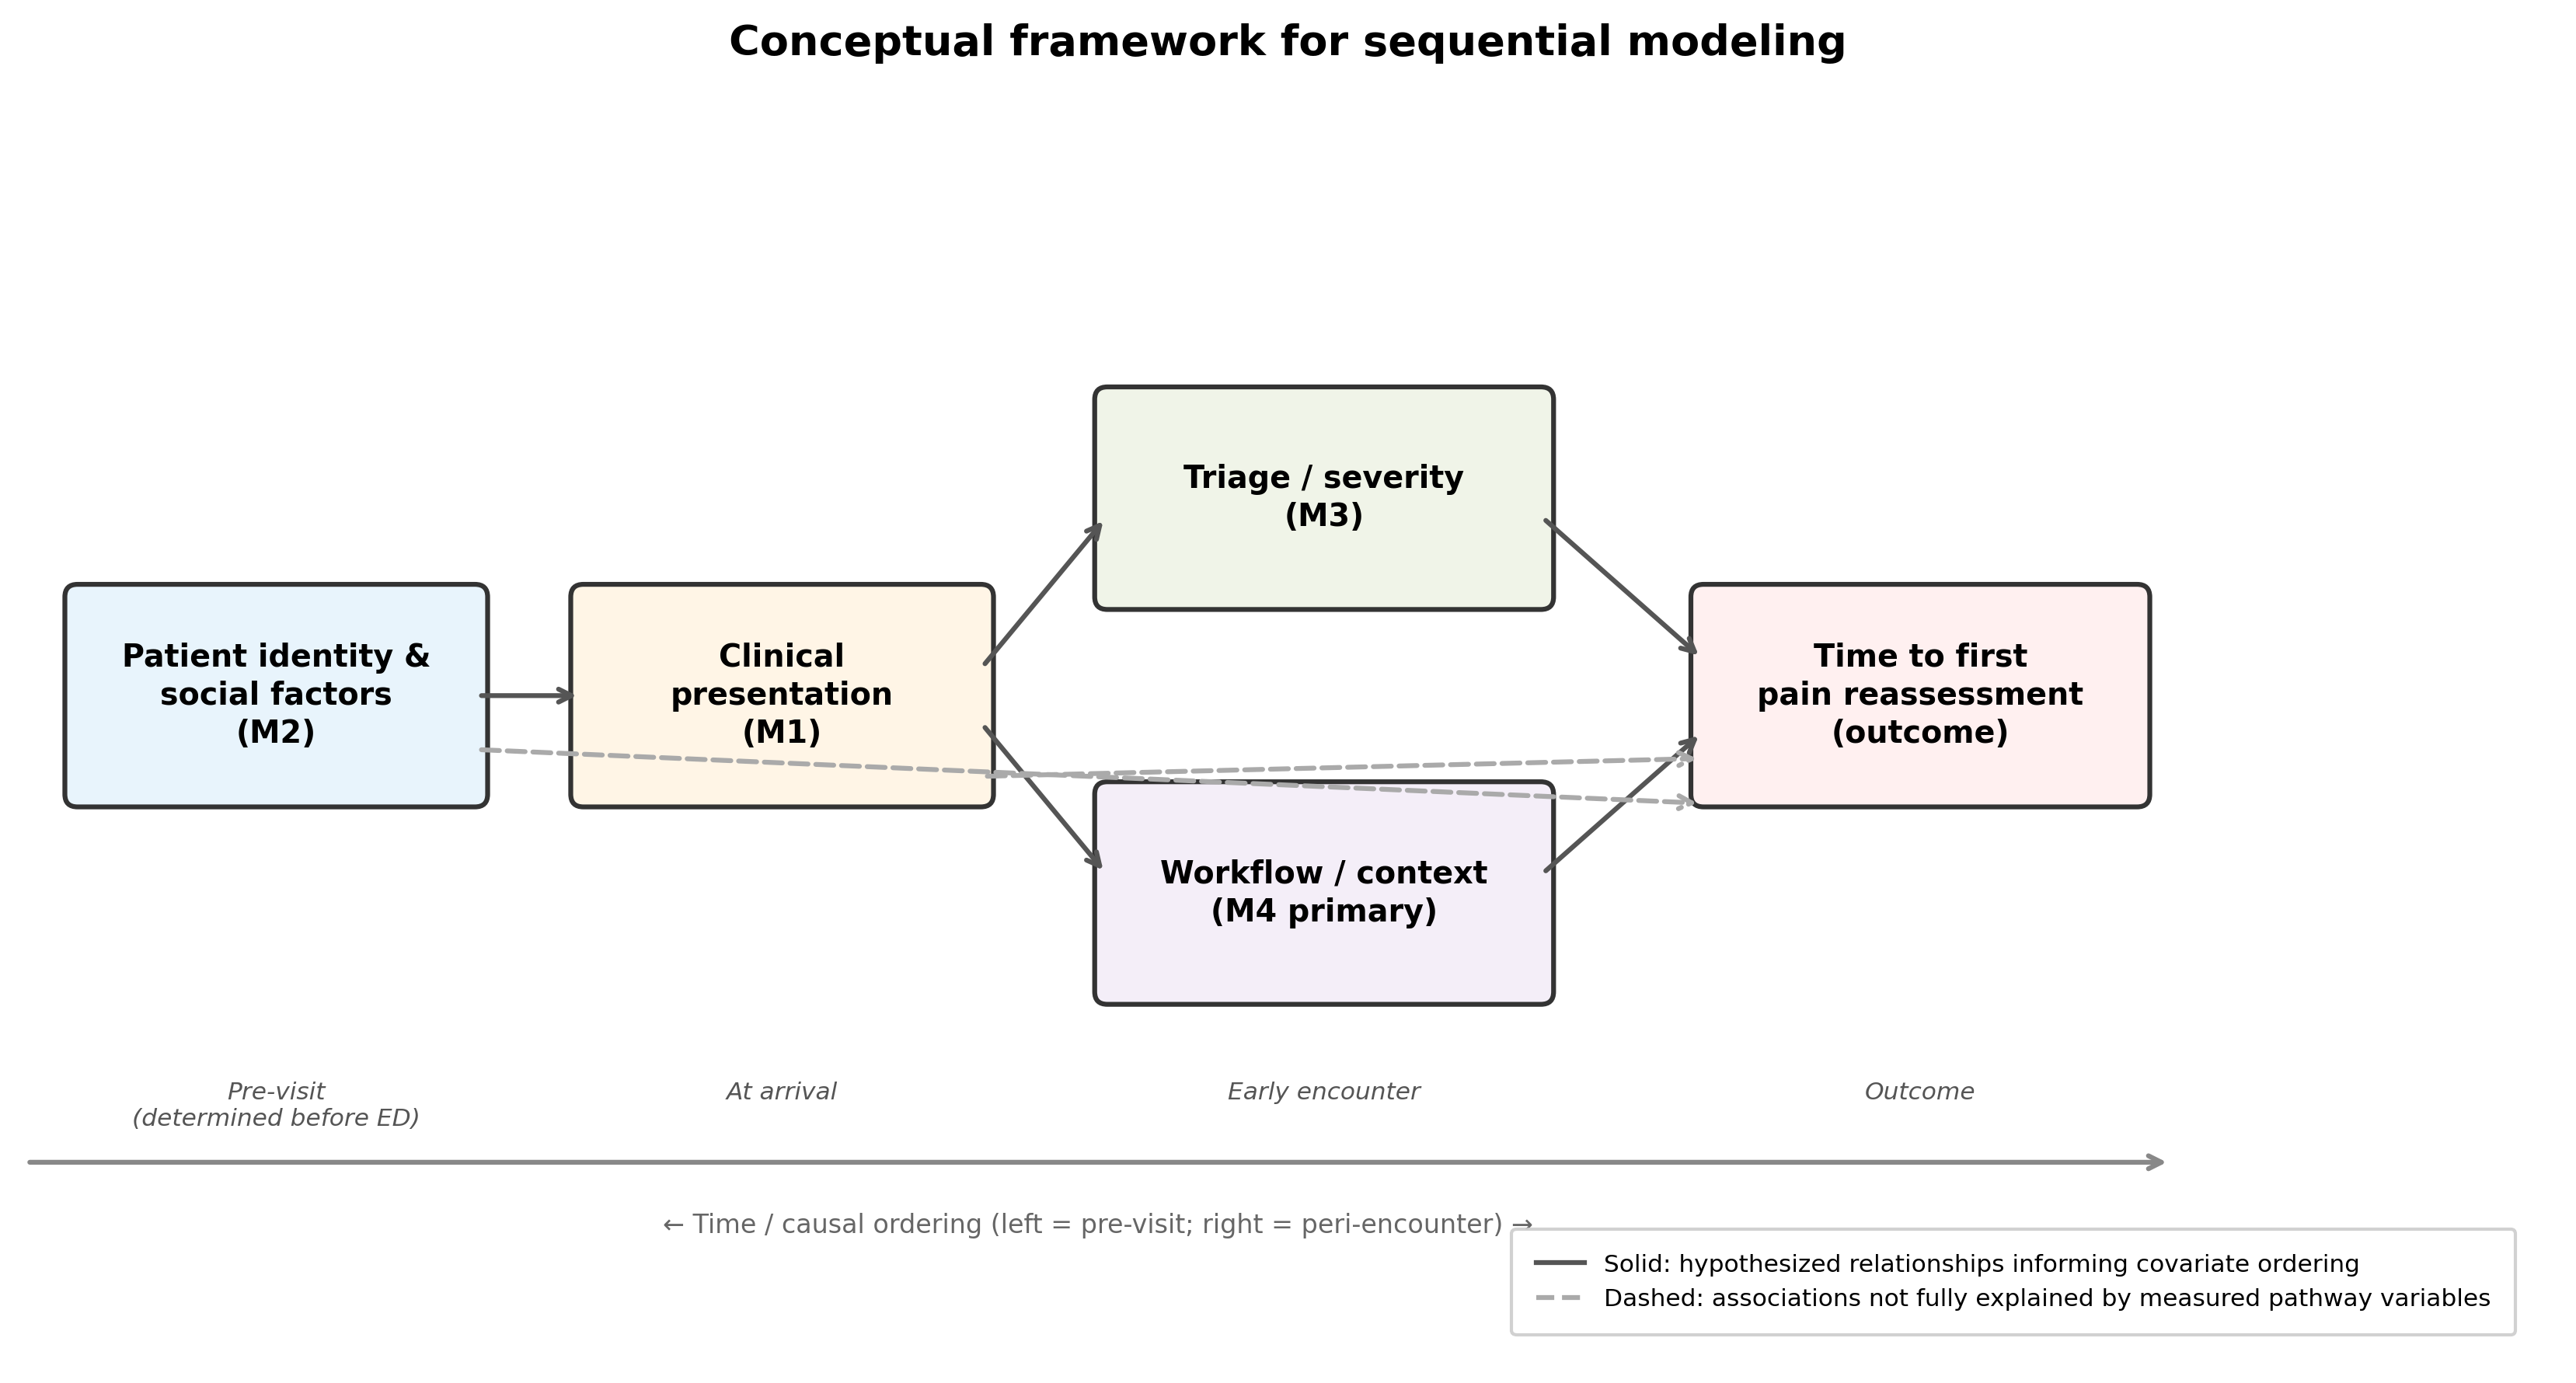
\includegraphics[width=\linewidth]{fig_main_conceptual_framework.png}
  \caption{Conceptual framework for sequential modeling.
  Boxes represent covariate domains arranged in hypothesized temporal order from left (patient identity and social factors determined before the visit) to right (ED workflow context).
  Solid arrows represent hypothesized relationships informing covariate ordering in the sequential models M1--M4; dashed arrows indicate associations not fully explained by measured pathway variables.
  Patient identity variables (M2) may relate to reassessment both through triage acuity, if equivalent presentations receive different ESI assignments depending on patient characteristics, and through pathways that bypass triage entirely.
  The sequential modeling strategy is designed to help distinguish these two routes: attenuation of a demographic coefficient after adding triage and severity covariates (M2 to M3) is consistent with triage- or severity-related pathways, while persistence across all models points to factors not captured by the measured covariates.
  This figure does not assert causal identification; it describes the conceptual basis for covariate sequencing.}
  \label{fig:dag}
\end{figure}

The framework encodes three key structural features.
First, initial pain score and diagnosis are upstream clinical signals that both trigger reassessment directly and inform triage acuity; they represent the \textit{clinical presentation} tier (M1).
Second, patient identity variables (insurance status, race/ethnicity, and preferred language) may relate to reassessment through two hypothesized routes: an indirect route operating through triage acuity (if patient identity shapes how clinical urgency is assigned) and a residual association not accounted for by triage.
Third, ESI triage acuity occupies an ambiguous structural position: it may act as a confounder (if it reflects true underlying severity that independently predicts reassessment), as a pathway variable (if the same clinical presentation receives different acuity assignments depending on patient identity), or both.
This ambiguity motivates the sequential modeling strategy described below, and is the reason we report results from models that progressively add covariate tiers rather than selecting a single adjusted specification.

ED operational factors (arrival mode, shift timing, and crowding) are downstream of both triage and patient identity.
Ambulance arrival in particular may lie on the pathway from insurance to reassessment (Medicaid patients are less likely to arrive by ambulance), and is therefore included in M4 as an operational covariate whose association should be interpreted as part of the care pathway rather than an independent confounder to be removed.

\subsection{Covariates and sequential model design}

Covariates were organized into four sequential tiers, each corresponding to a distinct phase of the care pathway and a distinct tier in Figure~\ref{fig:dag}:

\begin{itemize}
  \item \textbf{M1 (clinical presentation):} initial pain score (continuous) and injury/diagnosis group (acute pancreatitis as reference category). These variables represent the clinical signal that initiates the reassessment process: the patient's own report of their pain severity, and the clinical context in which it arises.

  \item \textbf{M2 (demographic and social factors):} race/ethnicity (White as reference; Black, Hispanic, and Asian), insurance (private as reference; Medicaid and Medicare), preferred language (English as reference when available), age group (18--39, 40--64 [reference], and 65+ years), and sex. These variables are upstream of triage assignment in the conceptual framework and represent patient characteristics that may shape how the clinical signal is received and acted upon, independent of its objective severity.

  \item \textbf{M3 (illness severity and triage):} ESI triage level, initial vital signs (heart rate, respiratory rate, and systolic blood pressure, each z-scored), and comorbidity count derived from linked ICD-based flags. As described in the conceptual framework, ESI occupies an ambiguous structural position. We include it at this tier to assess how much of the demographic associations in M2 are statistically accounted for by triage and severity covariates, while acknowledging that this adjustment may partially remove associations of interest in addition to controlling for confounding.

  \item \textbf{M4 (ED workflow context):} arrival mode (walk-in as reference), arrival shift (day shift as reference), weekend arrival, and ED crowding proxies: the number of new arrivals in the hour preceding the initial pain documentation and the total census at that hour. These variables capture operational conditions that vary across visits independently of patient characteristics and that may modify how quickly any given patient is monitored.
\end{itemize}

Two variable categories were intentionally excluded from the primary sequential models.
Disposition (admitted vs.\ discharged) occurs downstream of initial pain documentation and treatment decisions; including it would induce collider bias on the pathway between presentation and reassessment.
Analgesic treatment similarly falls between initial pain assessment and reassessment and is treated as a pathway variable in dedicated sensitivity analyses rather than a confounder.
Vital-sign coefficients are estimated in M3 and reported in the supplement; they are included for confounding control but are not the focus of primary inference.

\subsection{Statistical analysis}

We used Cox proportional hazards models to estimate hazard ratios (HRs) for time to first pain reassessment.
An HR greater than 1 indicates faster reassessment (shorter time to event); an HR less than 1 indicates slower reassessment.
We fit four models (M1 through M4) adding covariate tiers sequentially in the order above, with \textbf{M4} prespecified as the primary adjusted model for inference on demographic, insurance, and workflow associations.

The sequential structure serves an interpretive purpose beyond simple covariate adjustment.
The change in a coefficient from M2 to M3 indicates how much of a demographic association is statistically accounted for by triage- and severity-related covariates.
Because M3 introduces vital signs and comorbidity count alongside ESI, attenuation at this step is interpreted as consistent with triage- or severity-related pathways and is not attributed to ESI specifically; these models do not constitute a formal mediation analysis.
The change from M3 to M4 indicates additional attenuation through operational workflow factors.
Coefficients that remain stable across M3 and M4, as observed for insurance, indicate associations that are not explained by measured triage mix or operational context and may reflect structural or unmeasured factors in the care encounter.

Sequential attenuation was examined graphically for the three primary exposure variables (race/ethnicity, insurance, and initial pain score) across all four models (Figure~\ref{fig:attenuation}).

\paragraph{Additional analyses.}
\label{sec:sensitivity}
\begin{enumerate}
  \item \textbf{Within-acuity models:} M4-specification models fit separately within ESI strata (1--2, 3, and 4--5), to evaluate whether demographic associations persist after removing cross-stratum ESI variation entirely. This analysis addresses whether the insurance association reflects triage-level confounding not adequately controlled by including ESI as a continuous covariate.

  \item \textbf{Severe-pain sensitivity:} Primary analysis restricted to encounters with initial pain scores of 7--10 (and a secondary restriction to pain score 10 only), to evaluate whether findings hold among patients with unambiguously high self-reported pain burden.

  \item \textbf{Post-analgesic pathway analysis:} Time zero reset to the first analgesic administration after initial pain documentation, analyzing reassessment conditional on having received treatment. This analysis separates whether the system responds to a patient's initial pain report (primary outcome) from whether it monitors the response to treatment (post-analgesic outcome).

  \item \textbf{Year-over-year trend analysis:} Unadjusted and M4-adjusted probabilities of reassessment within 60 minutes compared across de-identified 5-year policy eras, with a supplementary continuous-year Cox model. This analysis evaluates whether reassessment documentation practices changed across the observation window.

  \item \textbf{Disposition pathway sensitivity:} M4 compared with M4 plus admitted-vs-home disposition as a covariate. Because disposition is a post-treatment variable, this model is not preferred for primary inference; it is reported to assess the degree to which disposition mediates workflow associations.

  \item \textbf{Inverse probability of treatment weighting (IPTW):} Medicaid versus private insurance comparison with propensity scores estimated using M1 through M3 covariates only (excluding workflow), as a complementary approach to assess robustness of the primary regression-based estimate.

  \item \textbf{Competing-risk sensitivity analysis (Fine--Gray):} The primary Cox model censors patients without reassessment at ED departure; this treats departure as non-informative censoring. To assess whether differential rates of early ED departure bias the primary estimates, we fit a Fine--Gray subdistribution hazard model \citep{Fine1999} treating ED departure without reassessment as a competing event (event code 2) and reassessment as the event of interest (event code 1). The full M4 covariate set was used. Subdistribution hazard ratios (sHRs) and cumulative incidence functions (Aalen--Johansen estimator) by insurance group are reported in Supplementary Table~\ref{tab:finegray} and Supplementary Figure~\ref{fig:finegray_cif}. Analysis was conducted in R~4.5.2 using the \texttt{cmprsk} package (version 2.2.12).
\end{enumerate}

Analyses were conducted in Python~3 using \texttt{lifelines} and \texttt{statsmodels}; code is available in the study repository (\texttt{scripts/run\_analysis.py}).

\subsection{Ethics}

MIMIC-IV-ED is a publicly available, de-identified database; credentialed users complete required training and data use agreements.
Institutional review board approval was not required for secondary analysis of de-identified data per the data use agreement.


\section{Results}
\label{sec:results}

\subsection{Cohort construction and characteristics}

Of \FlowAllED{} ED stays in the MIMIC-IV-ED extract, 47,773 carried an eligible acute pancreatitis or trauma diagnosis (10 excluded); 47,571 belonged to one of the four analyzed race/ethnicity categories (202 excluded); 29,502 had a positive initial pain score with valid time-to-event information (18,069 excluded); 29,263 had a documented ESI triage level (239 excluded); and \CohortN{} had documented insurance (12,059 excluded), forming the primary analytic cohort (Figure~\ref{fig:flow}).

\begin{figure}[htbp]
  \centering
  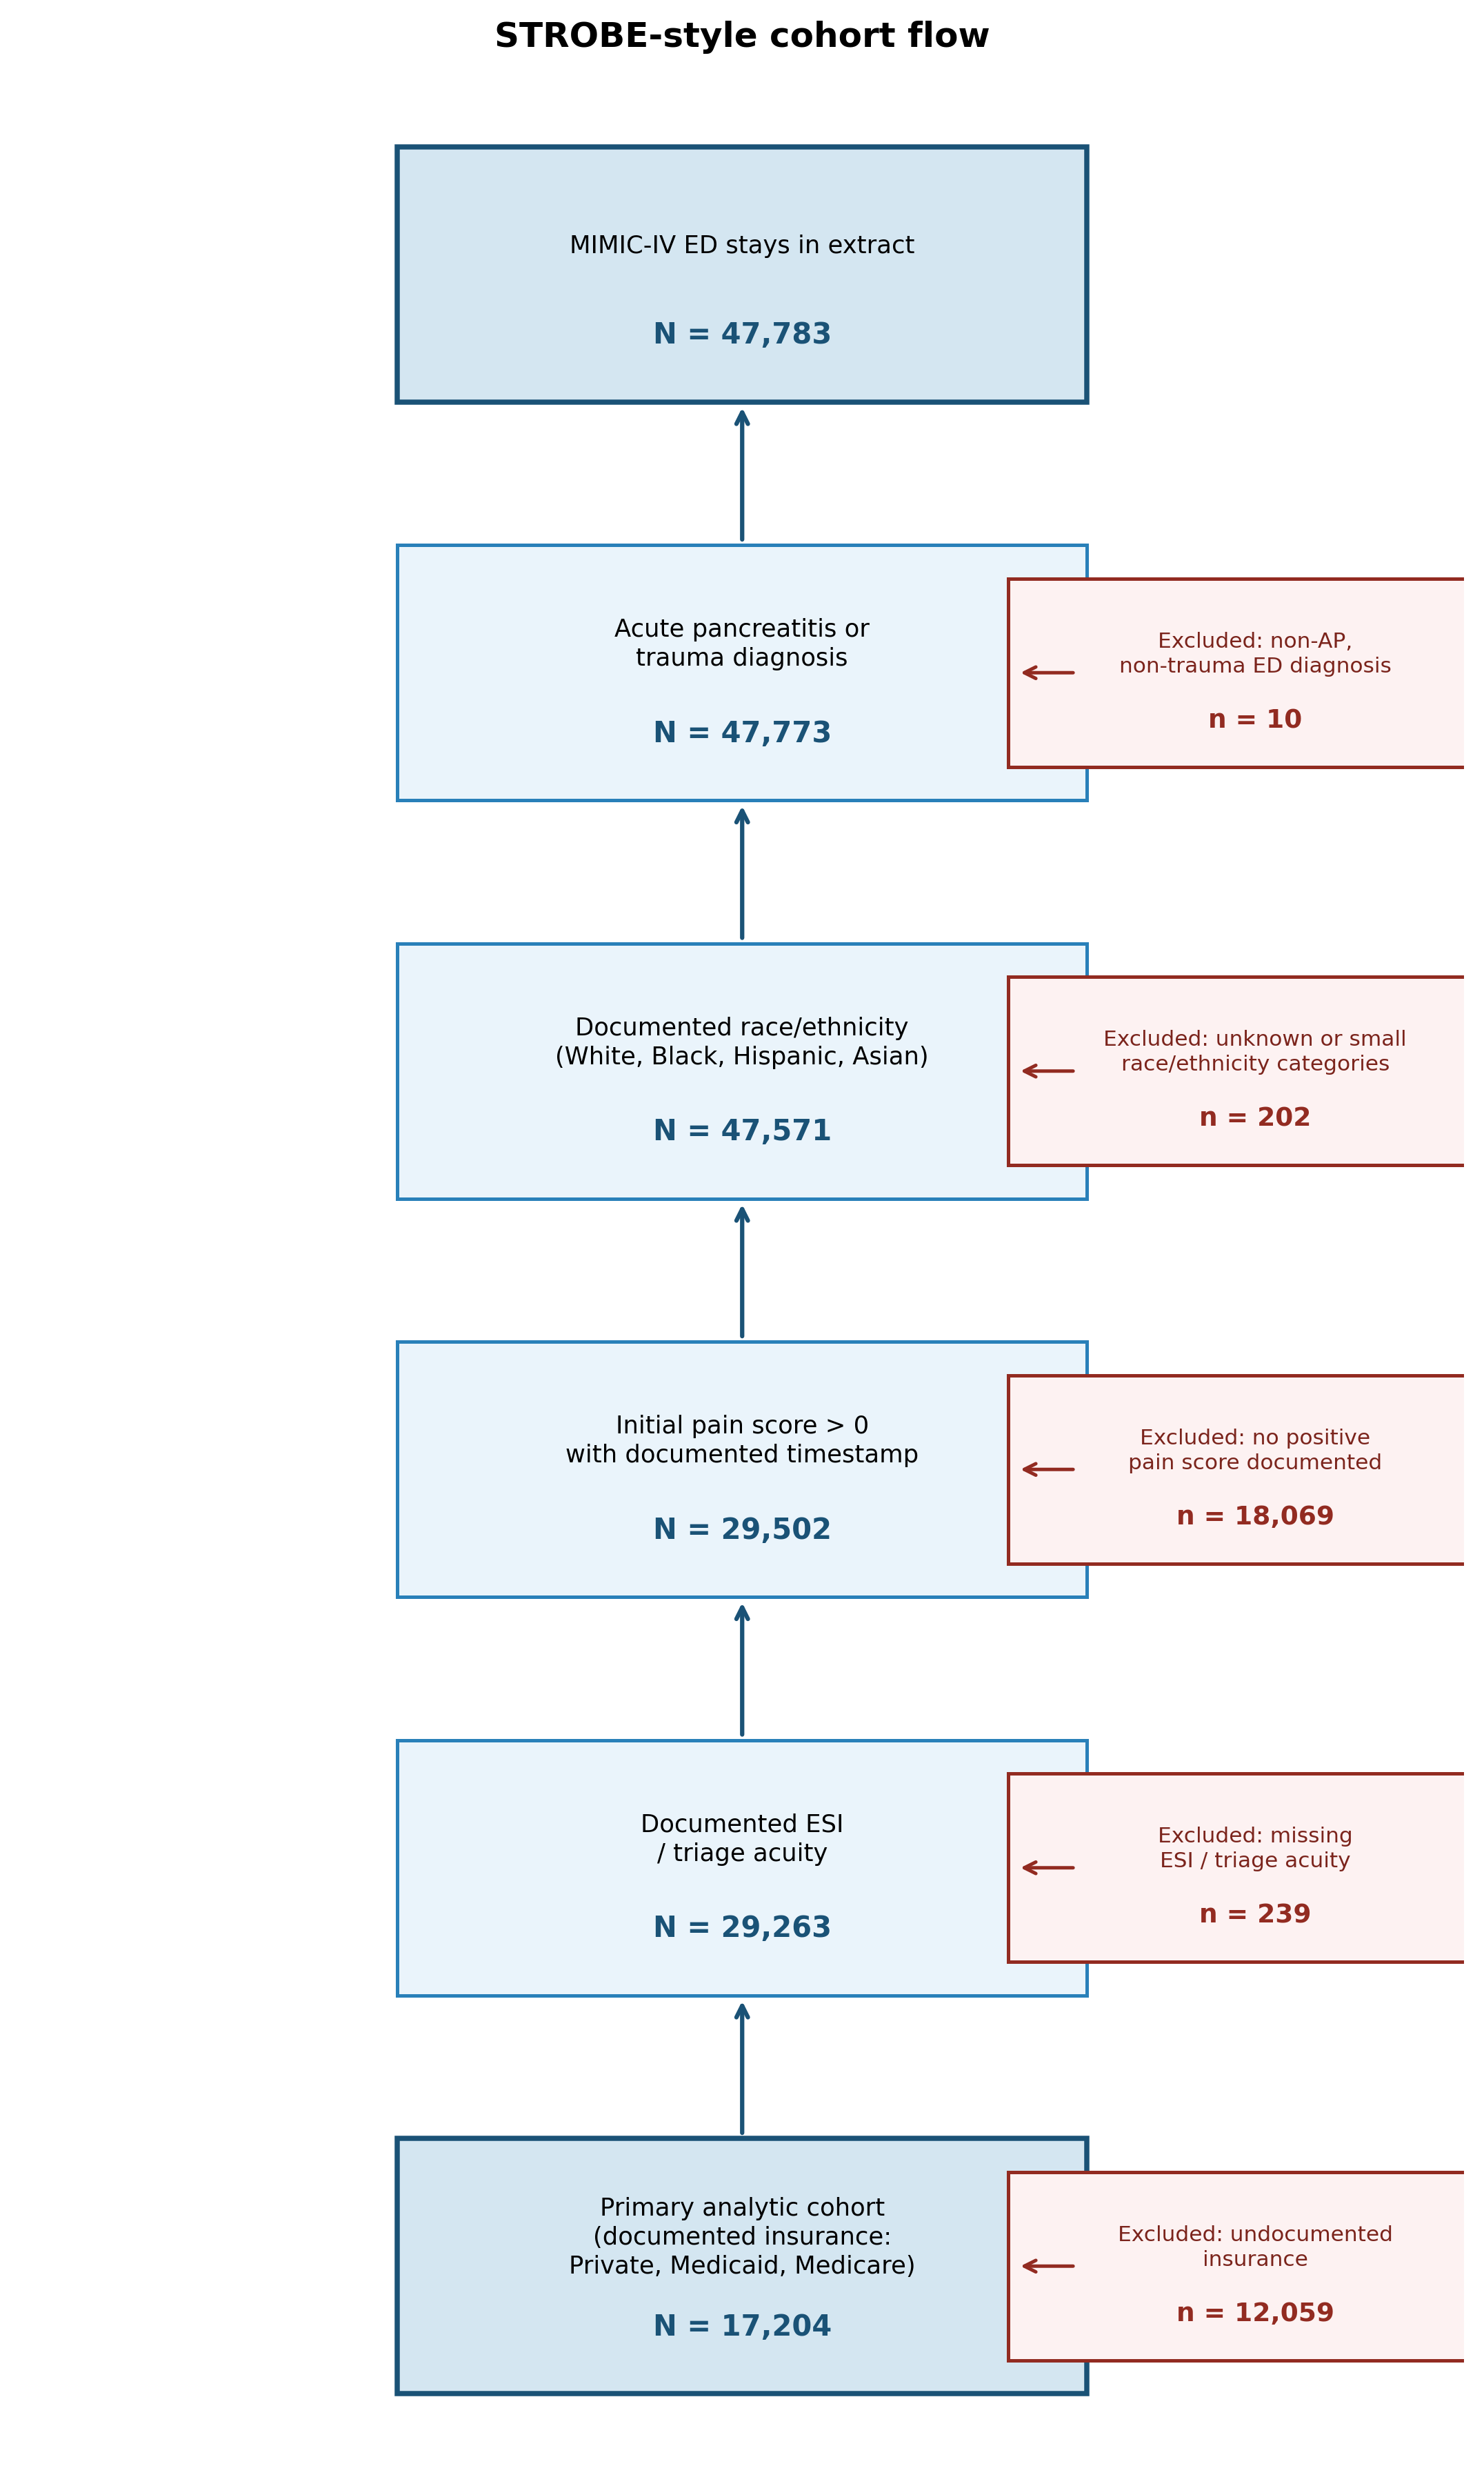
\includegraphics[width=0.85\linewidth]{fig_main_strobe_flow.png}
  \caption{STROBE-style cohort construction flow diagram. Boxes show the number of ED stays remaining after each inclusion criterion; exclusion counts appear in boxes branching to the right. Starting from \FlowAllED{} ED stays in the MIMIC-IV-ED extract, sequential exclusions yield the primary analytic cohort of \CohortN{} encounters.}
  \label{fig:flow}
\end{figure}

Of these \CohortN{} encounters, \CohortEvents{} (61.4\%) had at least one documented pain reassessment during the stay.
Cohort characteristics are shown in Table~\ref{tab:cohort}.
The mean age was 56.2 years (SD 19.7); 70.4\% of patients were White, 19.7\% Black, 6.9\% Hispanic, and 3.1\% Asian.
Most encounters were trauma-related (92.8\%); acute pancreatitis accounted for 7.2\%.
Insurance distribution was Medicare 46.6\%, private 29.5\%, and Medicaid 23.9\%.
Mean initial pain score was 6.1 (SD 2.6); mean ESI was 2.7 (SD 0.7).
Over half of patients arrived by ambulance (51.4\%); 8.0\% had a non-English preferred language.

\begin{table}[htbp]
\centering
\caption{Characteristics of the analytic cohort ($N=\CohortN{}$)}
\label{tab:cohort}
\footnotesize
\begin{tabular}{@{}lc@{}}
\toprule
Characteristic & Value \\
\midrule
\multicolumn{2}{@{}l}{\textit{Demographics}} \\
Age (years), mean (SD)            & 56.2 (19.7) \\
Female sex, $n$ (\%)              & 9,797 (56.9) \\
White race/ethnicity, $n$ (\%)    & 12,108 (70.4) \\
Black race/ethnicity, $n$ (\%)    & 3,383 (19.7) \\
Hispanic ethnicity, $n$ (\%)      & 1,186 (6.9) \\
Asian race/ethnicity, $n$ (\%)    & 527 (3.1) \\
\midrule
\multicolumn{2}{@{}l}{\textit{Insurance}} \\
Medicare, $n$ (\%)   & 8,015 (46.6) \\
Private, $n$ (\%)    & 5,071 (29.5) \\
Medicaid, $n$ (\%)   & 4,118 (23.9) \\
Non-English preferred language, $n$ (\%) & 1,380 (8.0) \\
\midrule
\multicolumn{2}{@{}l}{\textit{Clinical}} \\
ESI triage level, mean (SD)       & 2.7 (0.7) \\
Initial pain score, mean (SD)     & 6.1 (2.6) \\
Trauma diagnosis, $n$ (\%)        & 15,958 (92.8) \\
Acute pancreatitis, $n$ (\%)      & 1,246 (7.2) \\
\midrule
\multicolumn{2}{@{}l}{\textit{ED workflow}} \\
Ambulance arrival, $n$ (\%)       & 8,845 (51.4) \\
Weekend arrival, $n$ (\%)         & 4,907 (28.5) \\
Night shift arrival, $n$ (\%)     & 2,980 (17.3) \\
ED arrivals in prior hour, mean (SD) & 2.1 (1.3) \\
\midrule
\multicolumn{2}{@{}l}{\textit{Outcomes}} \\
Any reassessment, $n$ (\%)            & 10,569 (61.4) \\
Reassessed within 60 min, $n$ (\%)    & 1,651 (9.6) \\
Reassessed within 120 min, $n$ (\%)   & 3,722 (21.6) \\
Time to reassessment, median (IQR)    & 185 (96--311) min \\
\bottomrule
\end{tabular}
\end{table}


Reassessment was frequently delayed. The median time to first reassessment was 185 minutes (IQR 96--311).
Only 9.6\% of patients were reassessed within 60 minutes and 21.6\% within 120 minutes.
Unadjusted Kaplan--Meier curves showed separation by insurance and race/ethnicity (Figure~\ref{fig:km}); 60-minute reassessment rates varied by pain severity stratum (Figure~\ref{fig:rates60}).

\begin{figure}[htbp]
  \centering
  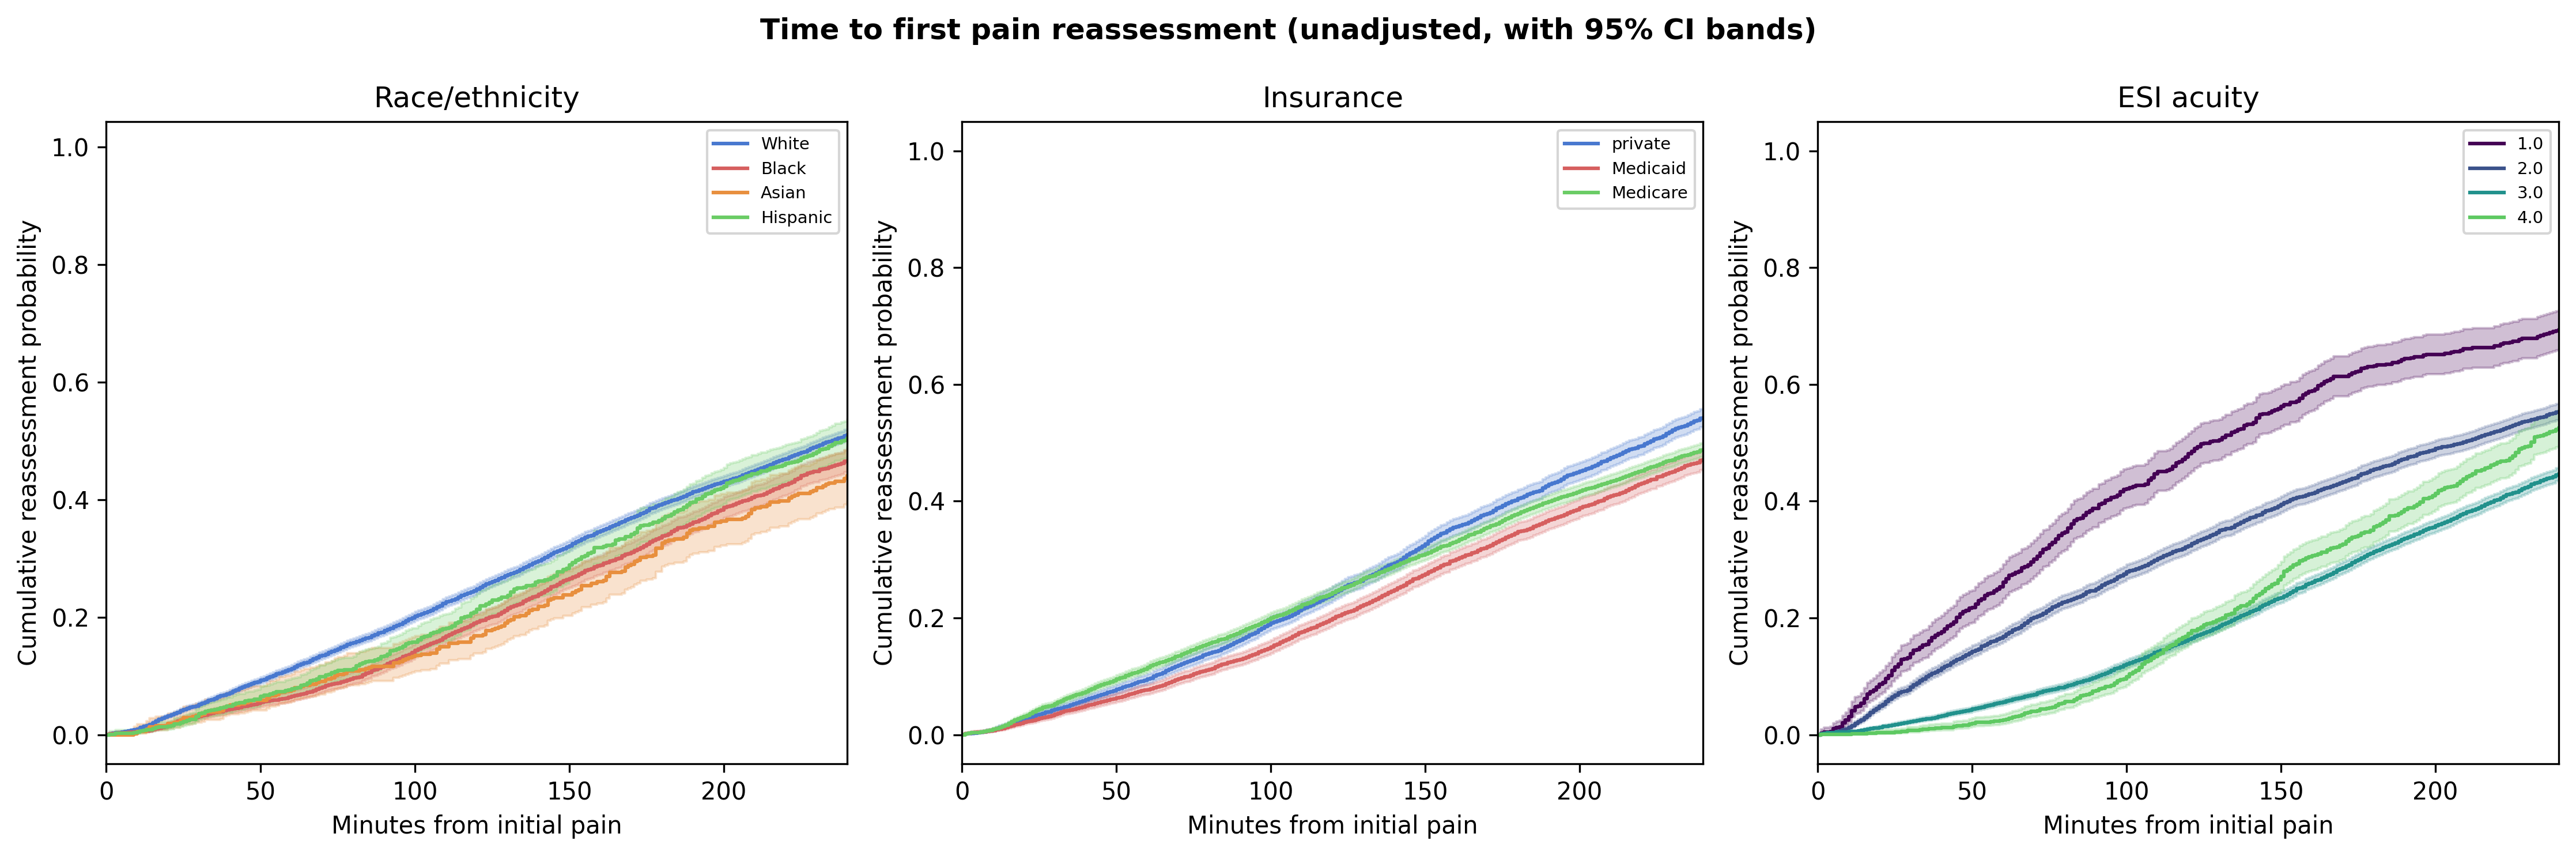
\includegraphics[width=\linewidth]{fig_main_km_ci.png}
  \caption{Unadjusted cumulative probability of first pain reassessment by race/ethnicity, insurance, and ESI triage level. Shaded bands represent pointwise 95\% confidence intervals (Greenwood formula).}
  \label{fig:km}
\end{figure}

\begin{figure}[htbp]
  \centering
  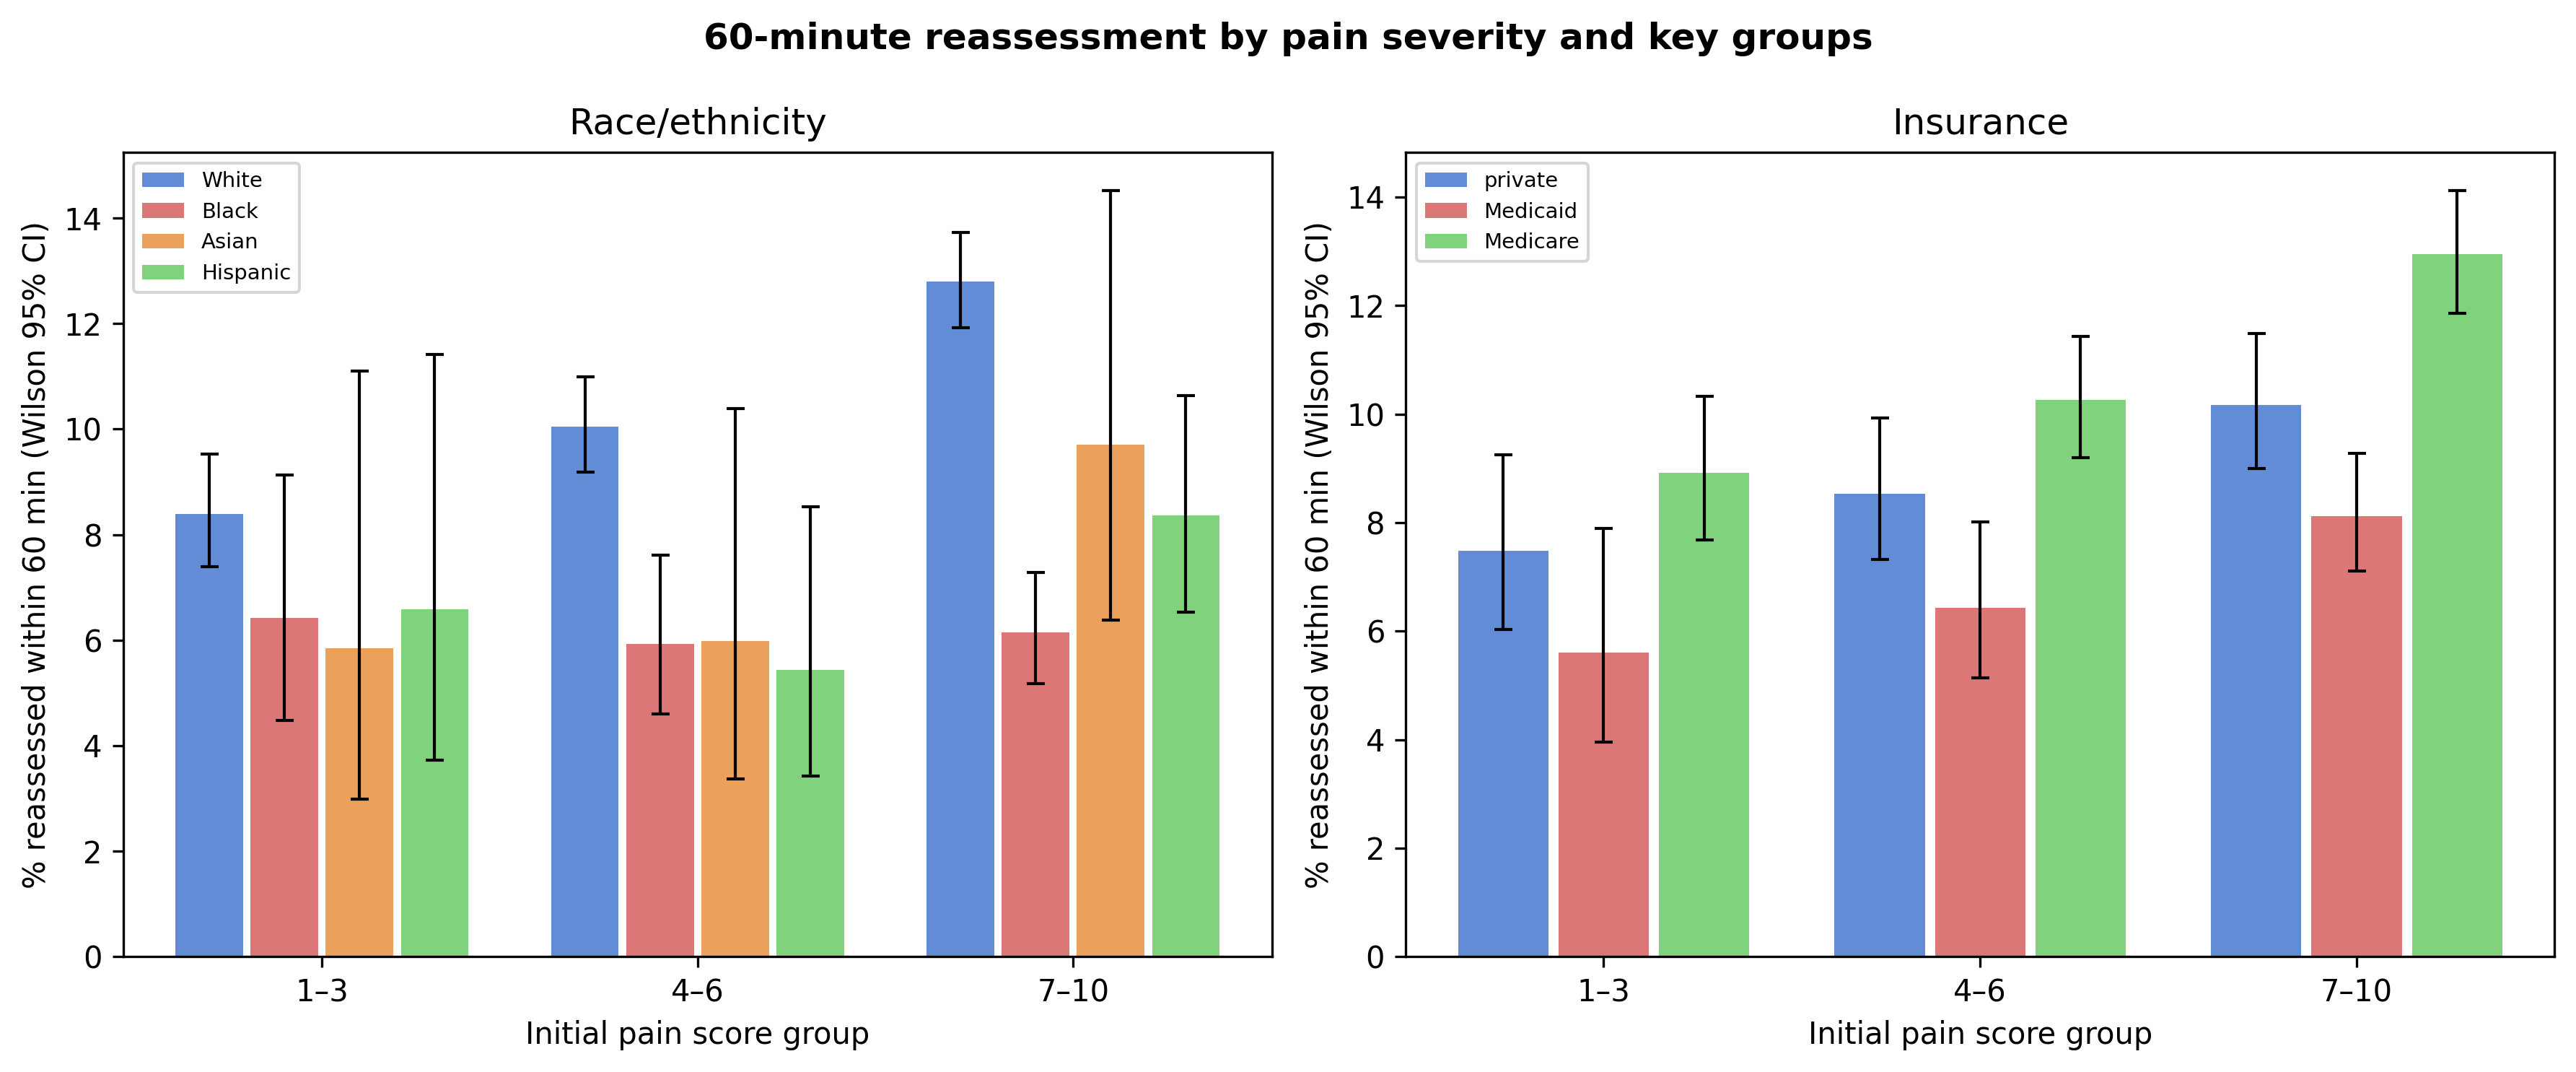
\includegraphics[width=0.9\linewidth]{fig_supp_60min_strata_ci.png}
  \caption{Unadjusted proportion reassessed within 60 minutes by initial pain severity group and race/ethnicity or insurance. Error bars show Wilson 95\% confidence intervals for proportions.}
  \label{fig:rates60}
\end{figure}

\subsection{Clinical presentation and reassessment timing}

In the primary adjusted M4 model (Figure~\ref{fig:m4forest}), clinical presentation variables showed the strongest and most clinically interpretable associations with reassessment timing.
Each one-point increase in initial pain score was associated with a faster rate of reassessment (HR \HRPainMfour{}): patients who reported higher pain were more likely to be checked on sooner, consistent with appropriate clinical prioritization of a patient's own symptom report.

Higher ESI level (lower triage acuity) was associated with substantially slower reassessment (HR \HRESIMfour{}).
This association reflects the central role of triage in organizing clinical attention: patients assigned lower acuity receive less intensive monitoring, and this association is large relative to most other covariates in the model.
As described in the Methods, ESI is interpreted here as both a clinically appropriate driver of monitoring intensity \textit{and} a potential pathway through which patient identity relates to reassessment (see Section~\ref{sec:race-esi-pathway} and Figure~\ref{fig:dag}).

\begin{figure}[htbp]
  \centering
  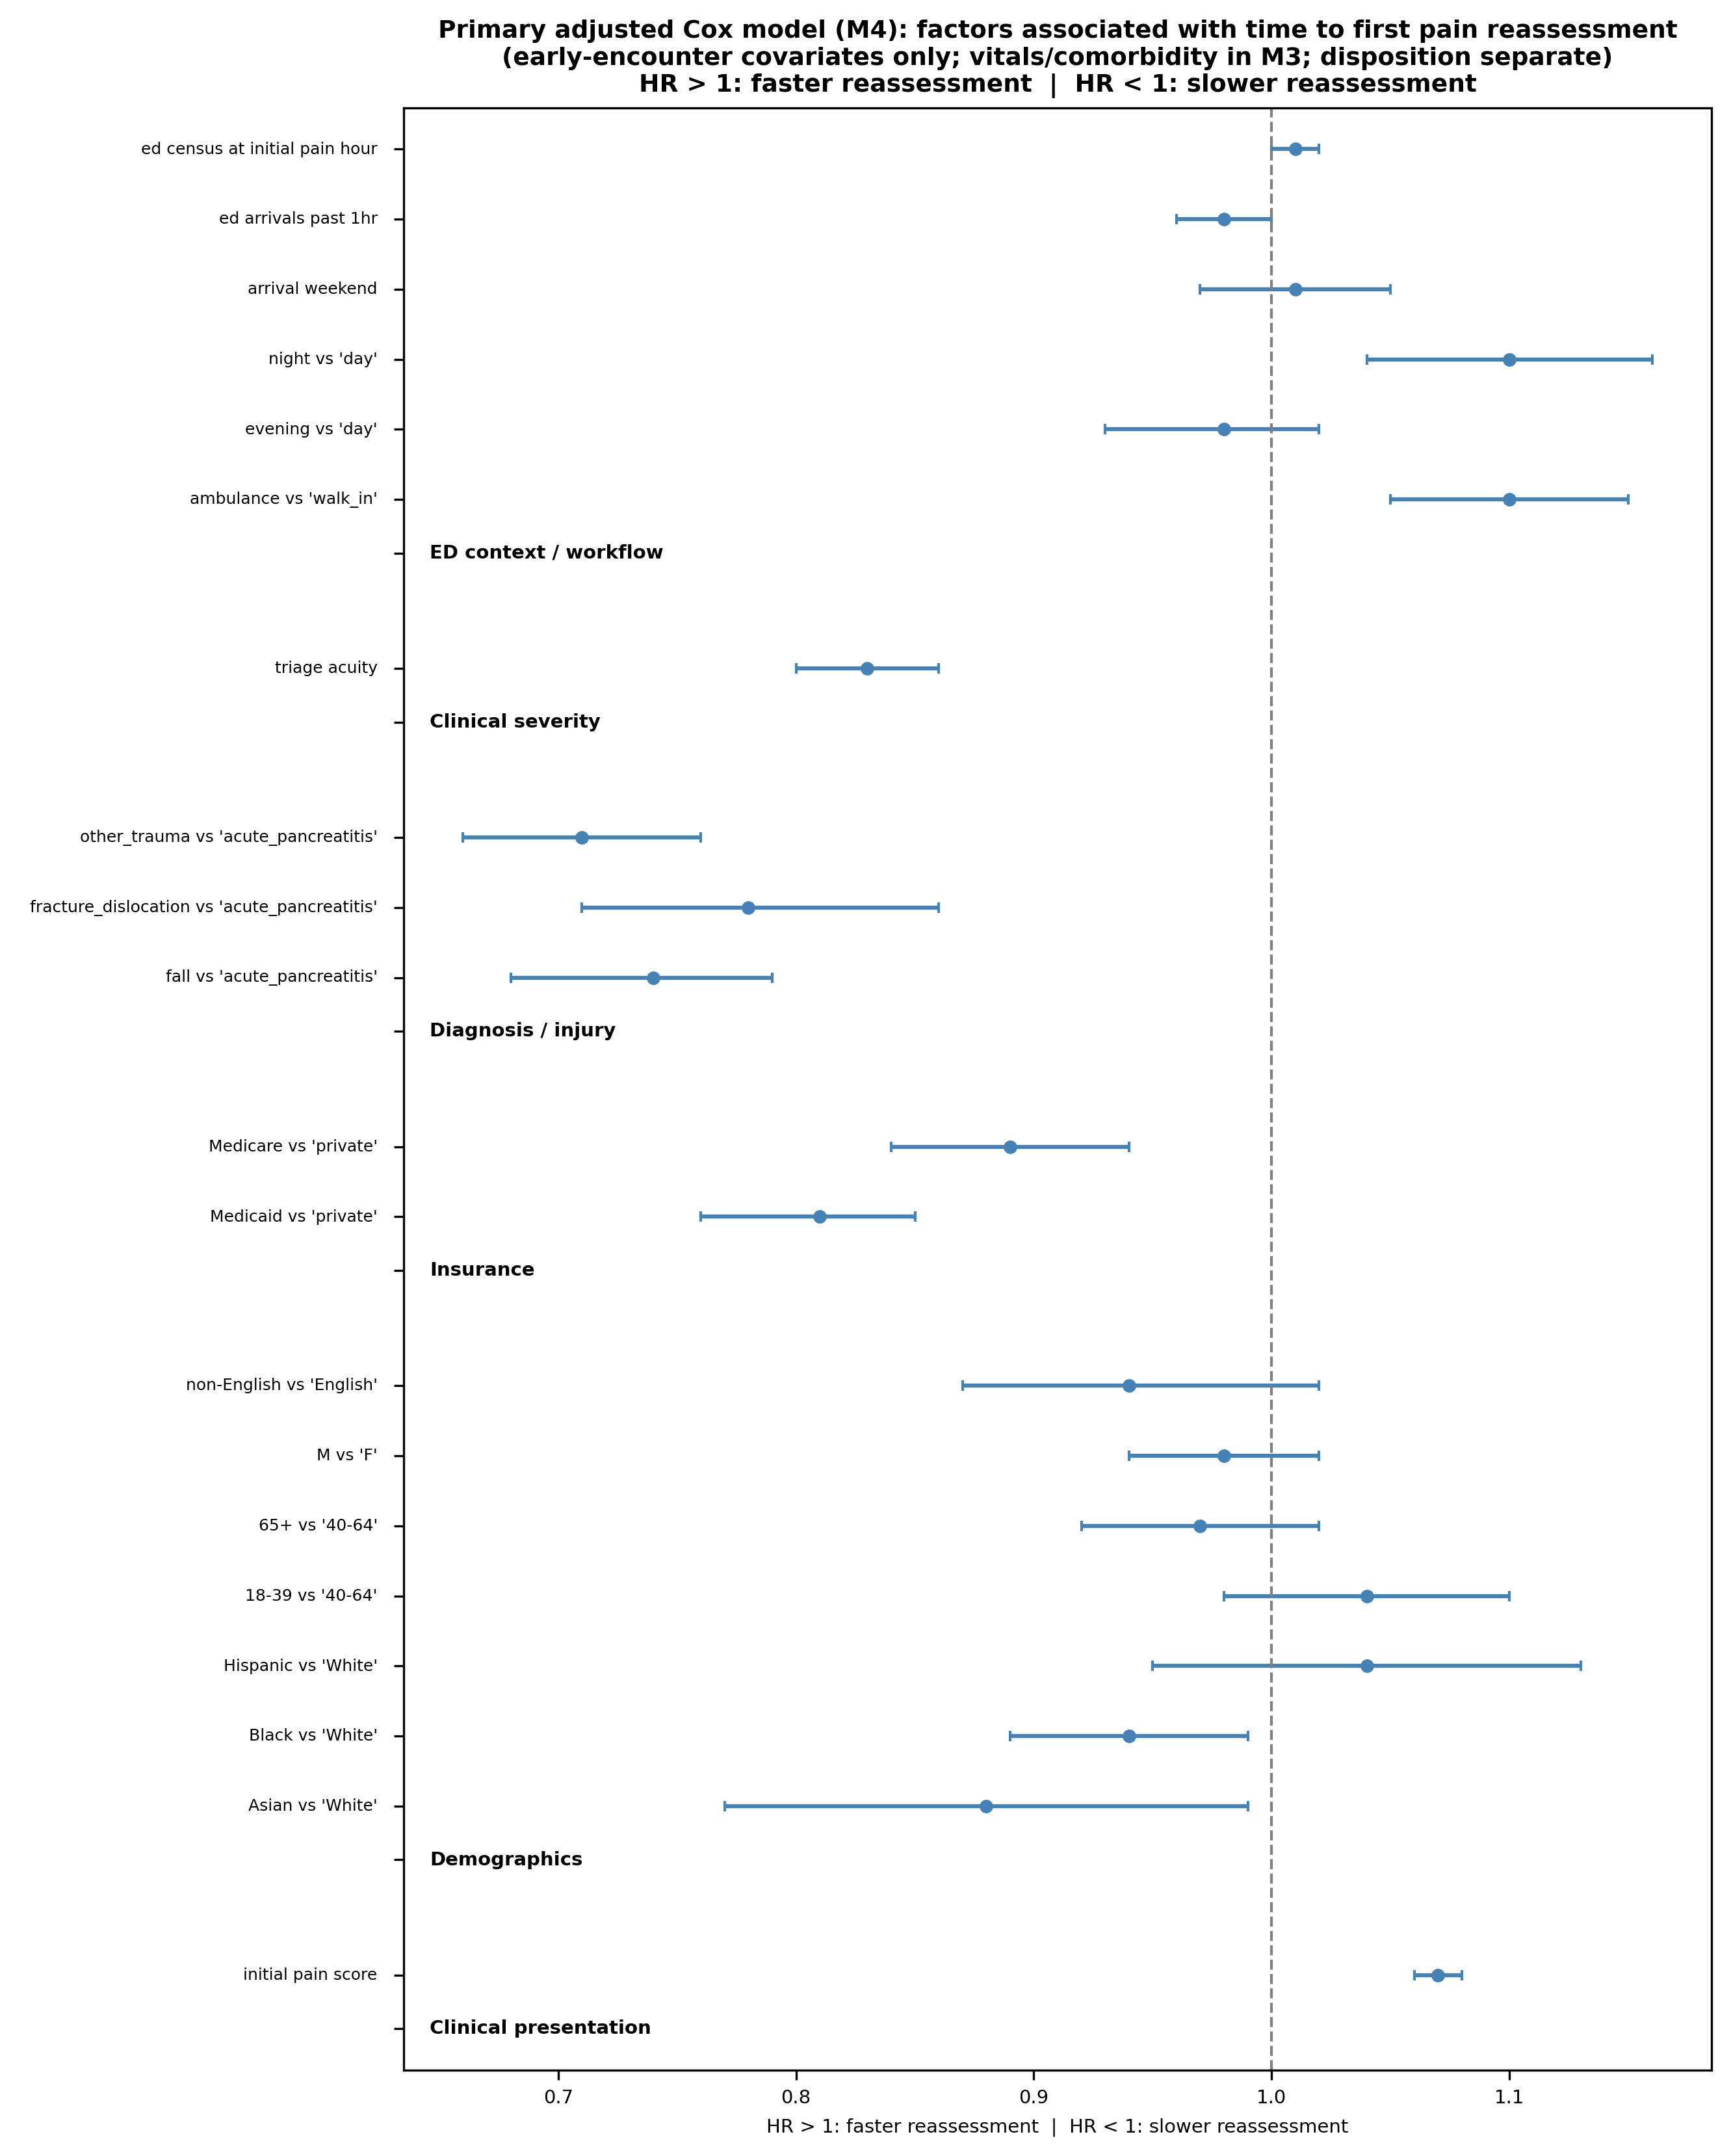
\includegraphics[width=0.95\linewidth]{fig_main_m4_forest.png}
  \caption{Primary adjusted Cox model (M4): hazard ratios for time to first pain reassessment.
  HR $>1$: faster reassessment; HR $<1$: slower reassessment.
  Vitals are adjusted in M3 but reported in the supplement; other arrival mode is excluded from the main panel.}
  \label{fig:m4forest}
\end{figure}

\subsection{Operational workflow factors}

Ambulance arrival was associated with faster reassessment compared with walk-in patients (HR \HRAmbulanceMfour{}), consistent with higher-acuity routing and more intensive initial evaluation for patients arriving by EMS.
Night shift was also associated with faster reassessment (HR \HRNightMfour{}), potentially reflecting lower census and staffing patterns that allow more frequent patient contact relative to the day shift.
Weekend arrival and ED crowding variables showed weaker or null associations at conventional significance thresholds, suggesting that short-term operational variation in volume may not substantially alter reassessment behavior within this cohort.

\subsection{Demographic pathways: race, ethnicity, and the role of triage}
\label{sec:race-esi-pathway}

Race and ethnicity showed associations with reassessment timing in earlier models that attenuated substantially with sequential adjustment (Figure~\ref{fig:attenuation}).
In M2 (demographic adjustment only), Black patients had slower reassessment than White patients (HR \HRBlackMtwo{}).
This association attenuated toward the null after adding ESI and severity covariates in M3, and remained modest in the fully adjusted M4 model (HR \HRBlackMfour{}).
Hispanic patients showed no meaningful association in any model (HR \HRHispanicMfour{}).
Asian patients had slower reassessment in M4 (HR \HRAsianMfour{}), but confidence intervals widened in severe-pain sensitivity analyses, limiting the precision of this estimate.

This pattern of attenuation requires careful interpretation rather than indicating simply that demographic associations disappear with adjustment.
The conceptual framework (Figure~\ref{fig:dag}) encodes the hypothesis that patient characteristics may shape triage acuity assignment: if identical clinical presentations receive different ESI levels depending on who the patient is, then ESI functions partly as a pathway variable rather than a confounder to be removed.
Because M3 introduces vital signs and comorbidity count alongside ESI, the attenuation cannot be attributed to ESI specifically; the pattern is consistent with race/ethnicity-related associations being partly embedded in triage and severity assessment.
Under this interpretation, the residual M4 coefficient reflects the association remaining after adjustment for measured triage- and severity-related pathways, not the total difference between groups.

\begin{figure}[htbp]
  \centering
  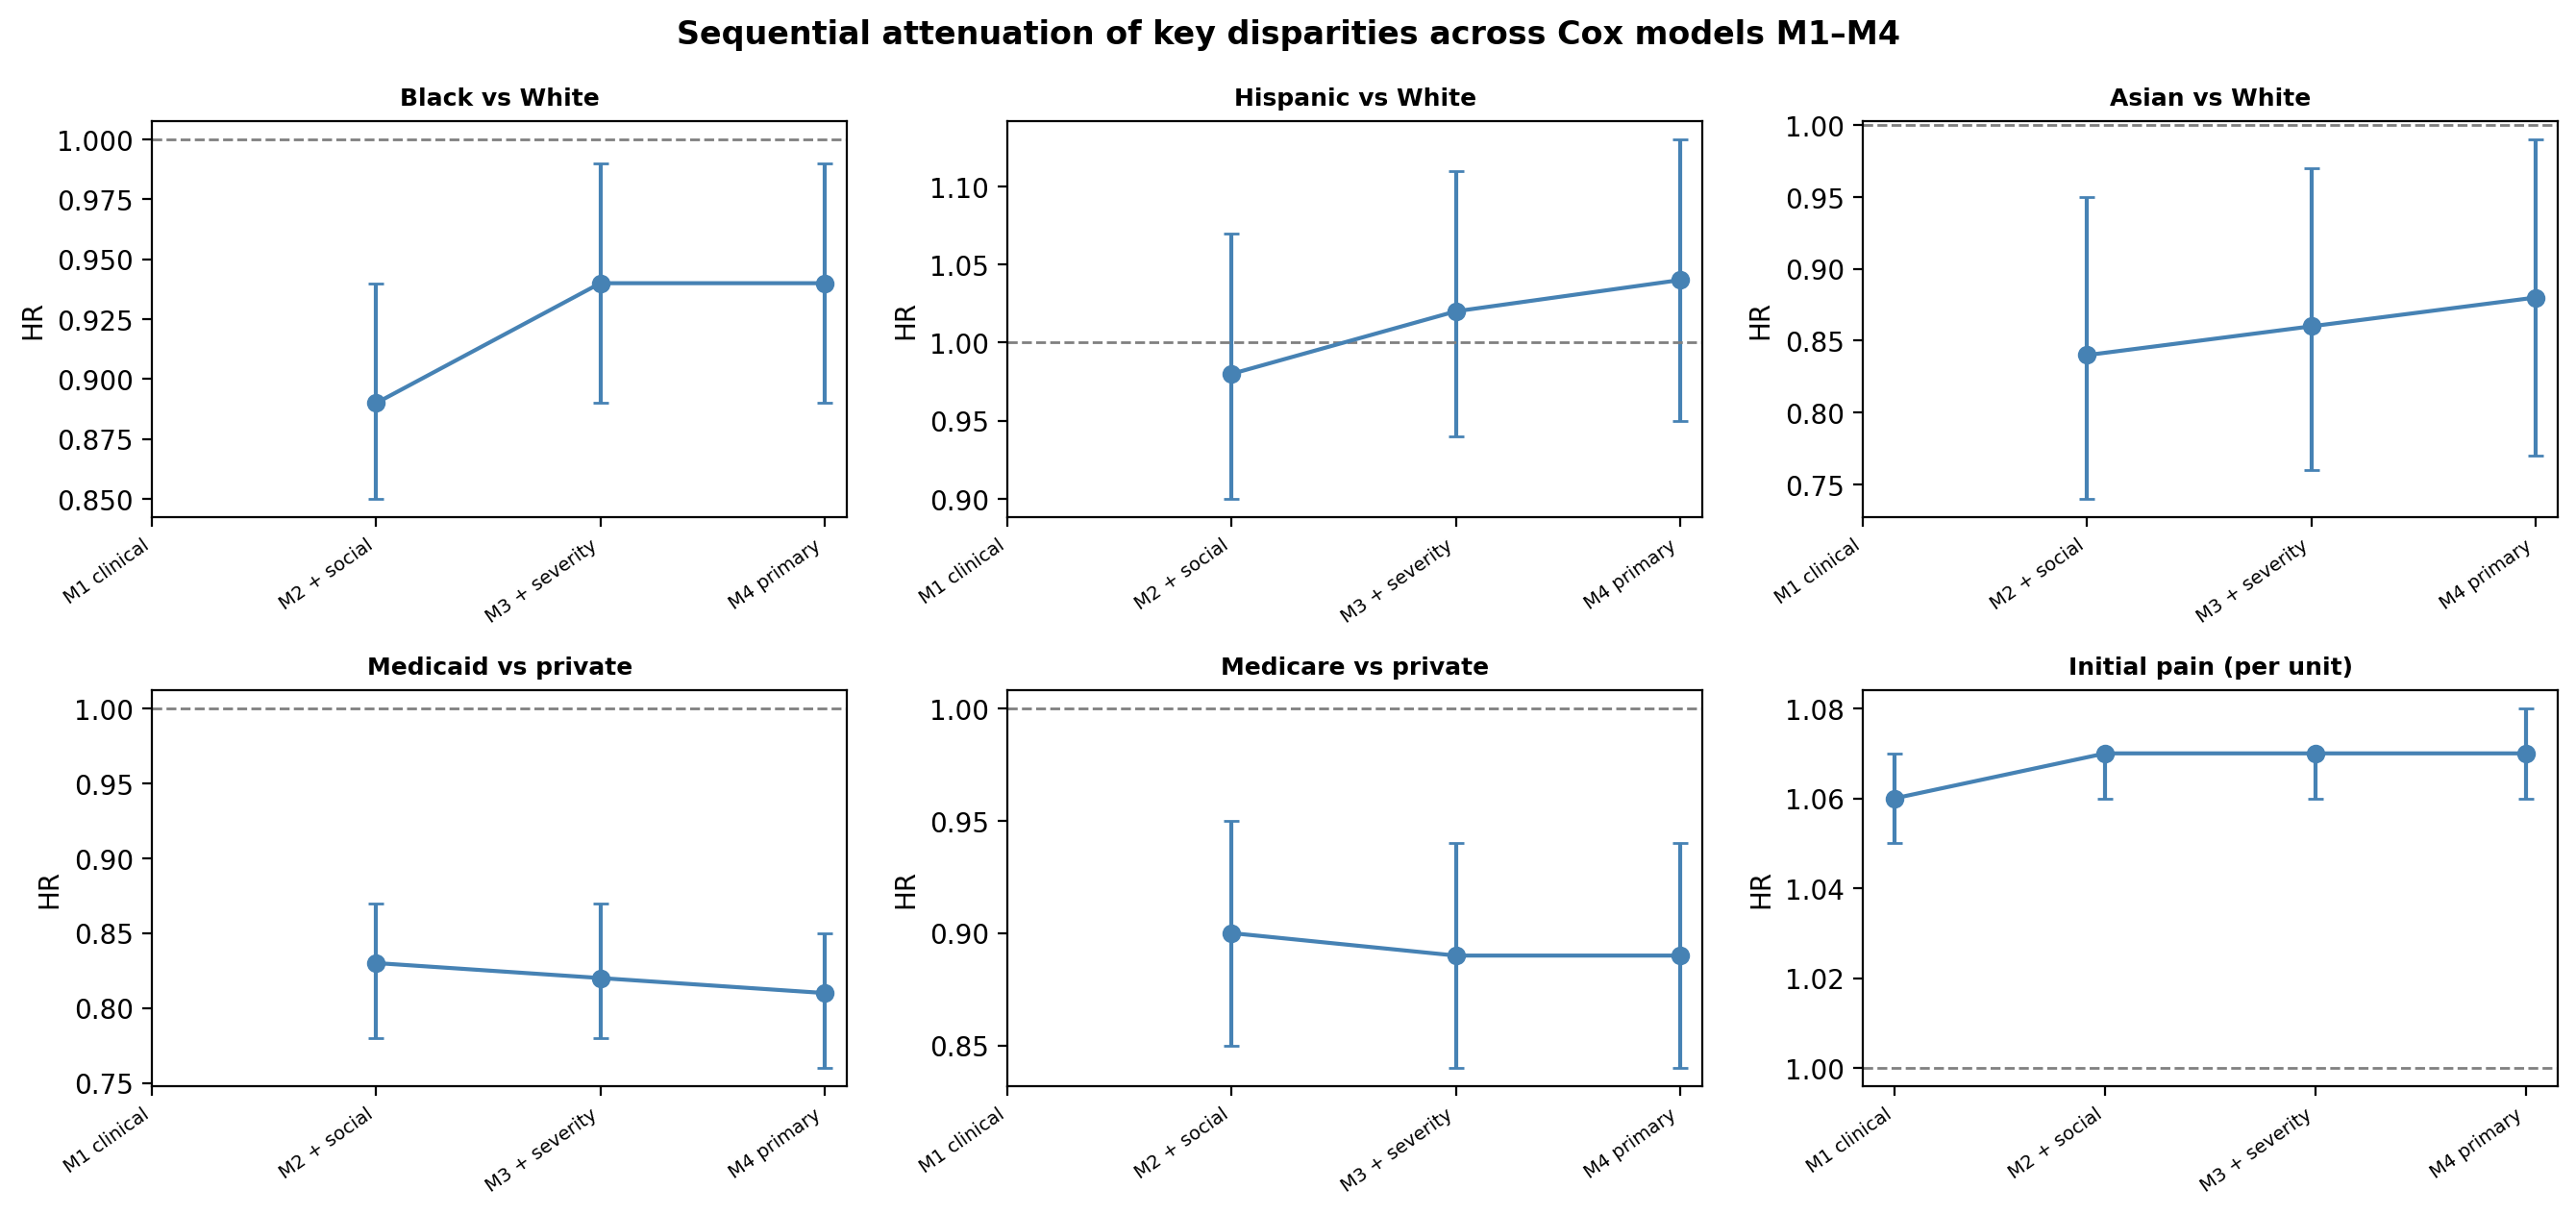
\includegraphics[width=\linewidth]{fig_main_sequential_attenuation.png}
  \caption{Sequential attenuation of race/ethnicity, insurance, and initial pain across models M1--M4.}
  \label{fig:attenuation}
\end{figure}

\subsection{Insurance: a persistent association not explained by measured clinical or triage factors}

Insurance showed the largest and most stable associations with reassessment timing among the social and demographic variables.
Compared with private insurance, Medicaid was associated with substantially slower reassessment in the fully adjusted model (HR \HRMedicaidMfour{}), representing approximately a 20\% lower instantaneous rate of reassessment throughout the ED stay.
Medicare was also associated with slower reassessment (HR \HRMedicareMfour{}), though the magnitude was smaller than for Medicaid.

In contrast to the race/ethnicity findings, the Medicaid association showed minimal attenuation across sequential models: from M2 (\HRMedicaidMtwo{}) through M3 (\HRMedicaidMthree{}) to M4 (\HRMedicaidMfourSeq{}).
Medicaid status was thus a stable marker of slower documented reassessment, not accounted for by measured differences in triage acuity, clinical severity, arrival mode, or shift distribution between Medicaid and privately insured patients (see Figure~\ref{fig:dag}, dashed arrow).

Within-acuity analyses corroborated this pattern (Figure~\ref{fig:insurance}).
Among ESI 1--2 encounters, Medicaid patients were reassessed more slowly than privately insured patients (HR \HRMedicaidESIhigh{}).
Among ESI 3 encounters, Medicaid remained associated with slower reassessment (HR \HRMedicaidESImed{}).
Estimates in ESI 4--5 were imprecise due to smaller event counts.
The persistence of the insurance association even among the highest-acuity patients argues against the explanation that Medicaid patients are simply lower-acuity on average.

\begin{figure}[htbp]
  \centering
  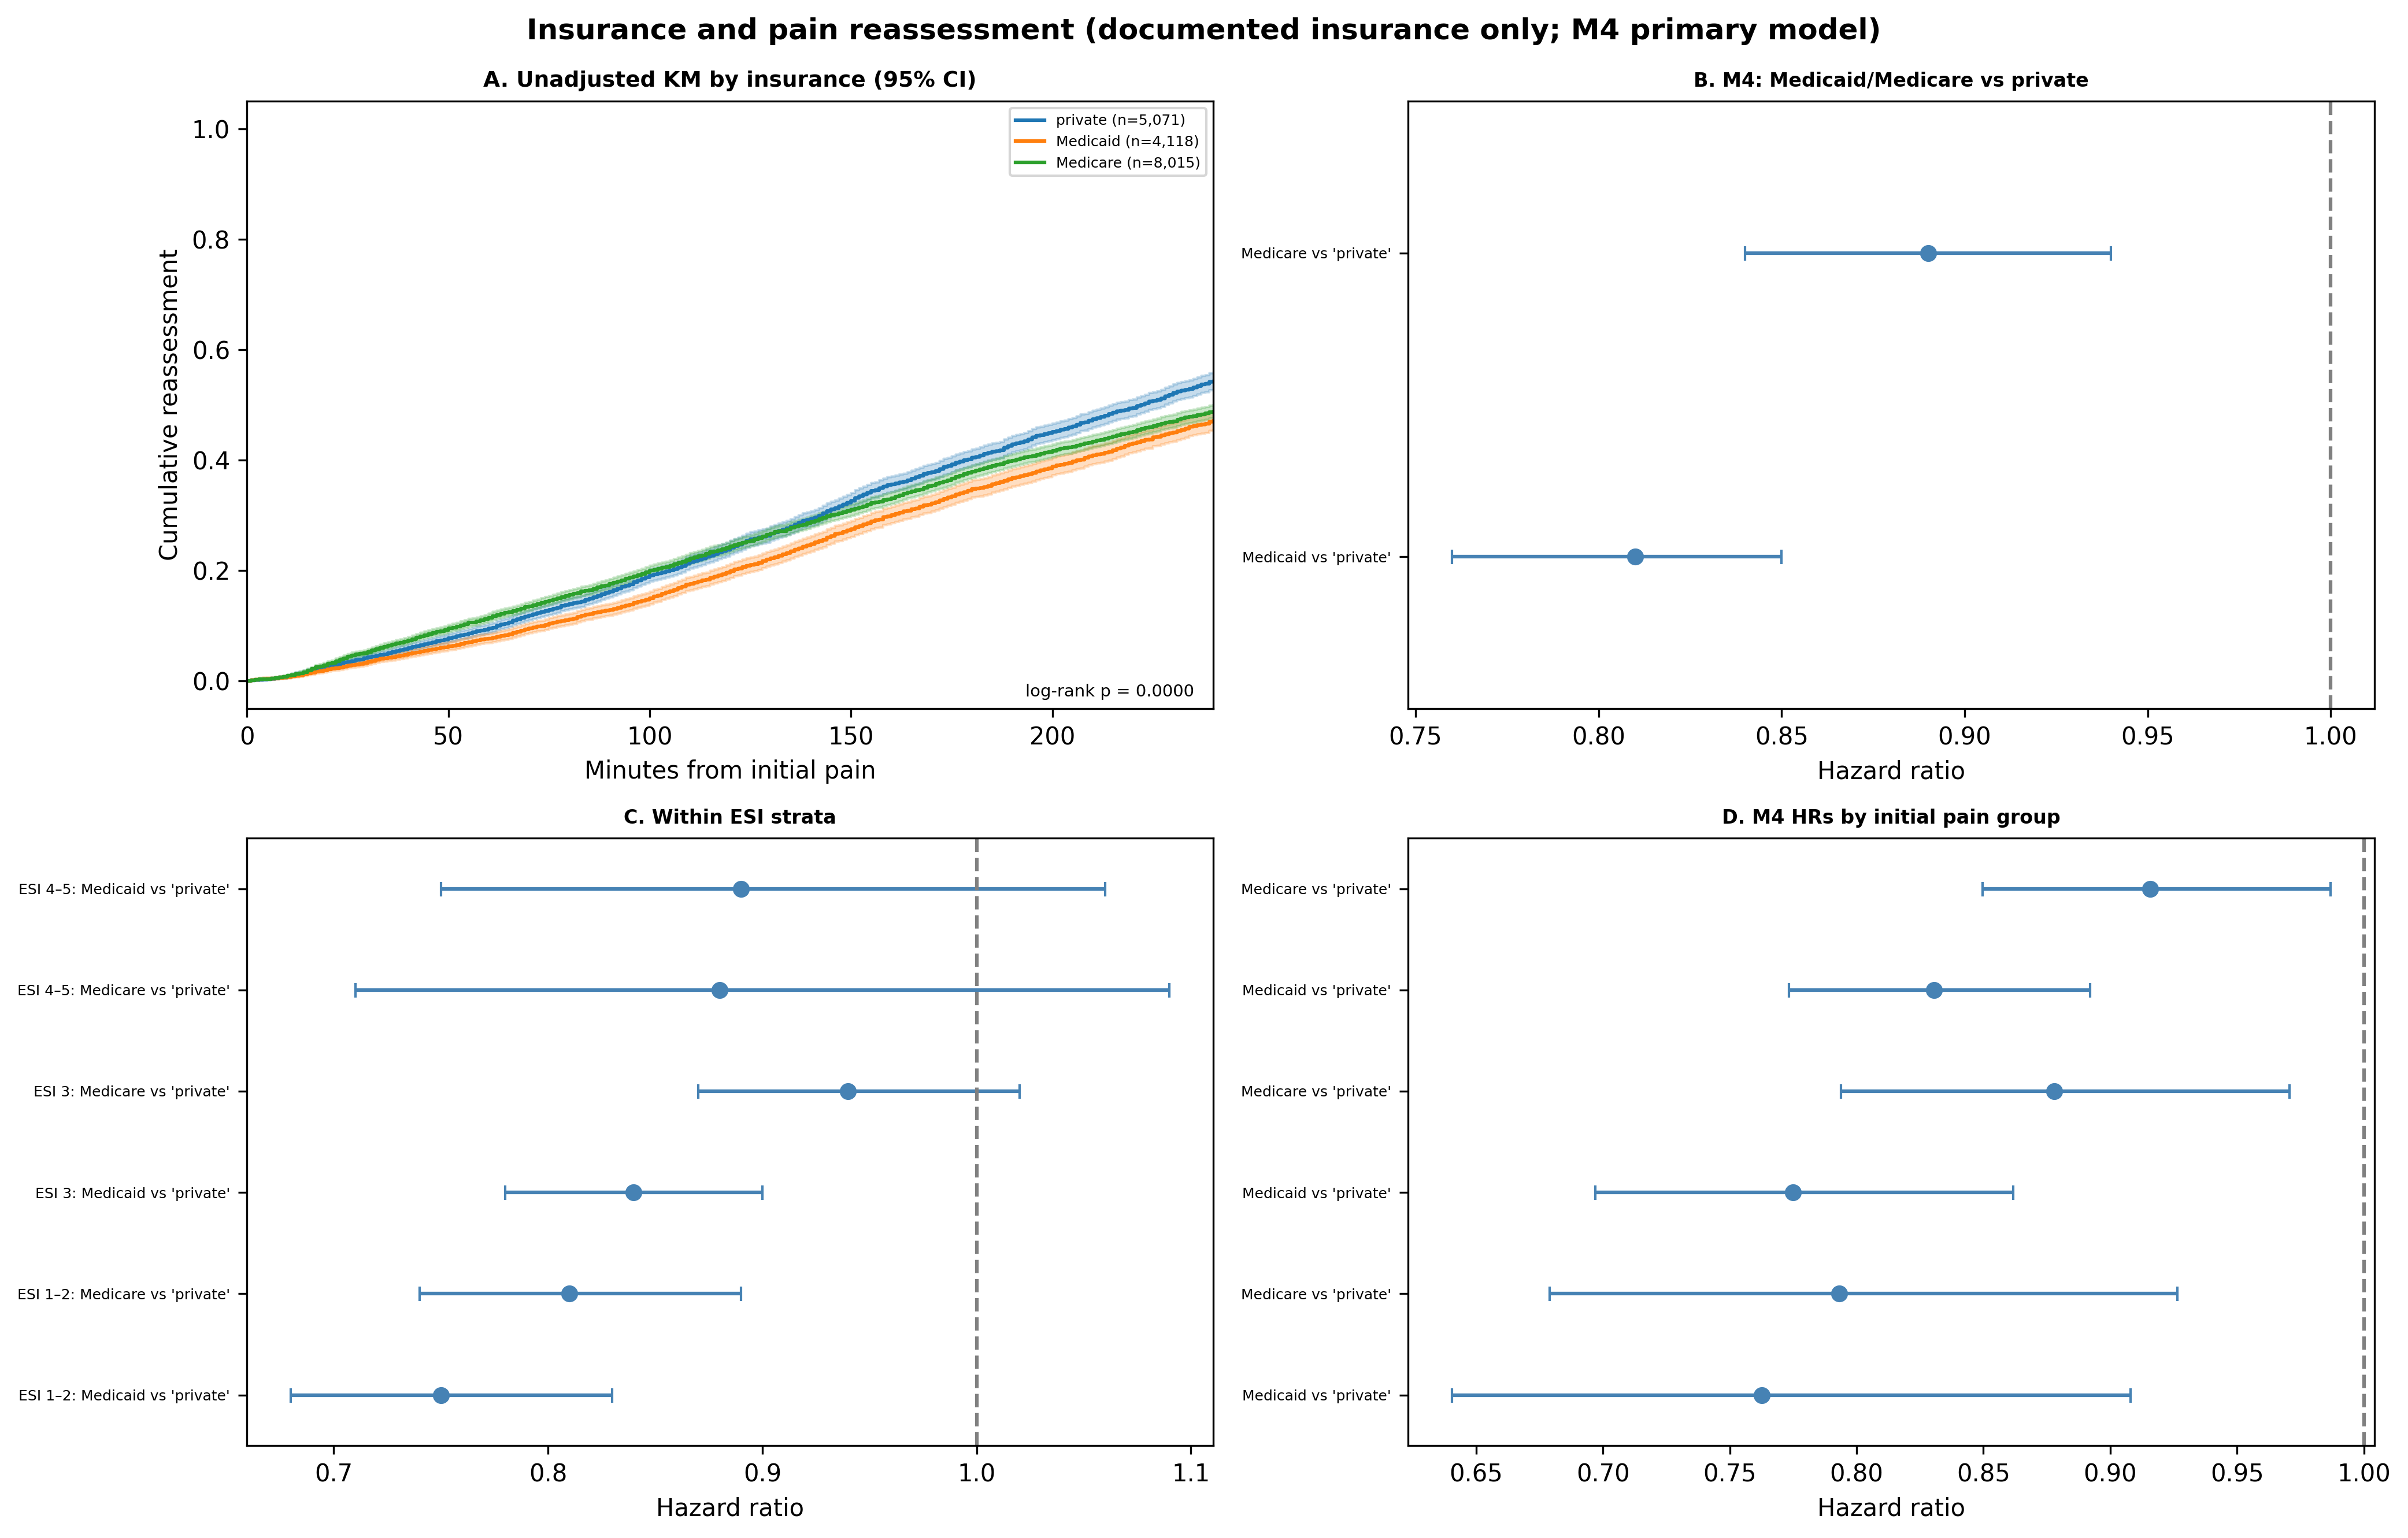
\includegraphics[width=\linewidth]{fig_main_insurance_panel.png}
  \caption{Insurance-focused analysis: unadjusted curves, M4 hazard ratios, within-acuity Medicaid estimates, and pain-stratum models.}
  \label{fig:insurance}
\end{figure}

\subsection{Severe-pain and within-acuity sensitivity analyses}

Among patients reporting severe pain (initial pain score 7--10), an insurance-based difference in reassessment persisted (HR \HRMedicaidSevere{}).
These are patients whose self-reported symptom burden should, if the system were responding to the clinical signal alone, uniformly trigger monitoring.
The persistence of the insurance gradient in this subgroup cannot be attributed to Medicaid patients reporting lower pain or being perceived as lower-acuity, because this restriction excludes those patients entirely.

Within-acuity models showed a similar pattern (Figure~\ref{fig:withinacuity}).
The Black--White difference in the severe-pain subgroup was HR \HRBlackSevere{}, consistent with the primary analysis and subject to the same triage-pathway interpretation described in Section~\ref{sec:race-esi-pathway}.

\begin{figure}[htbp]
  \centering
  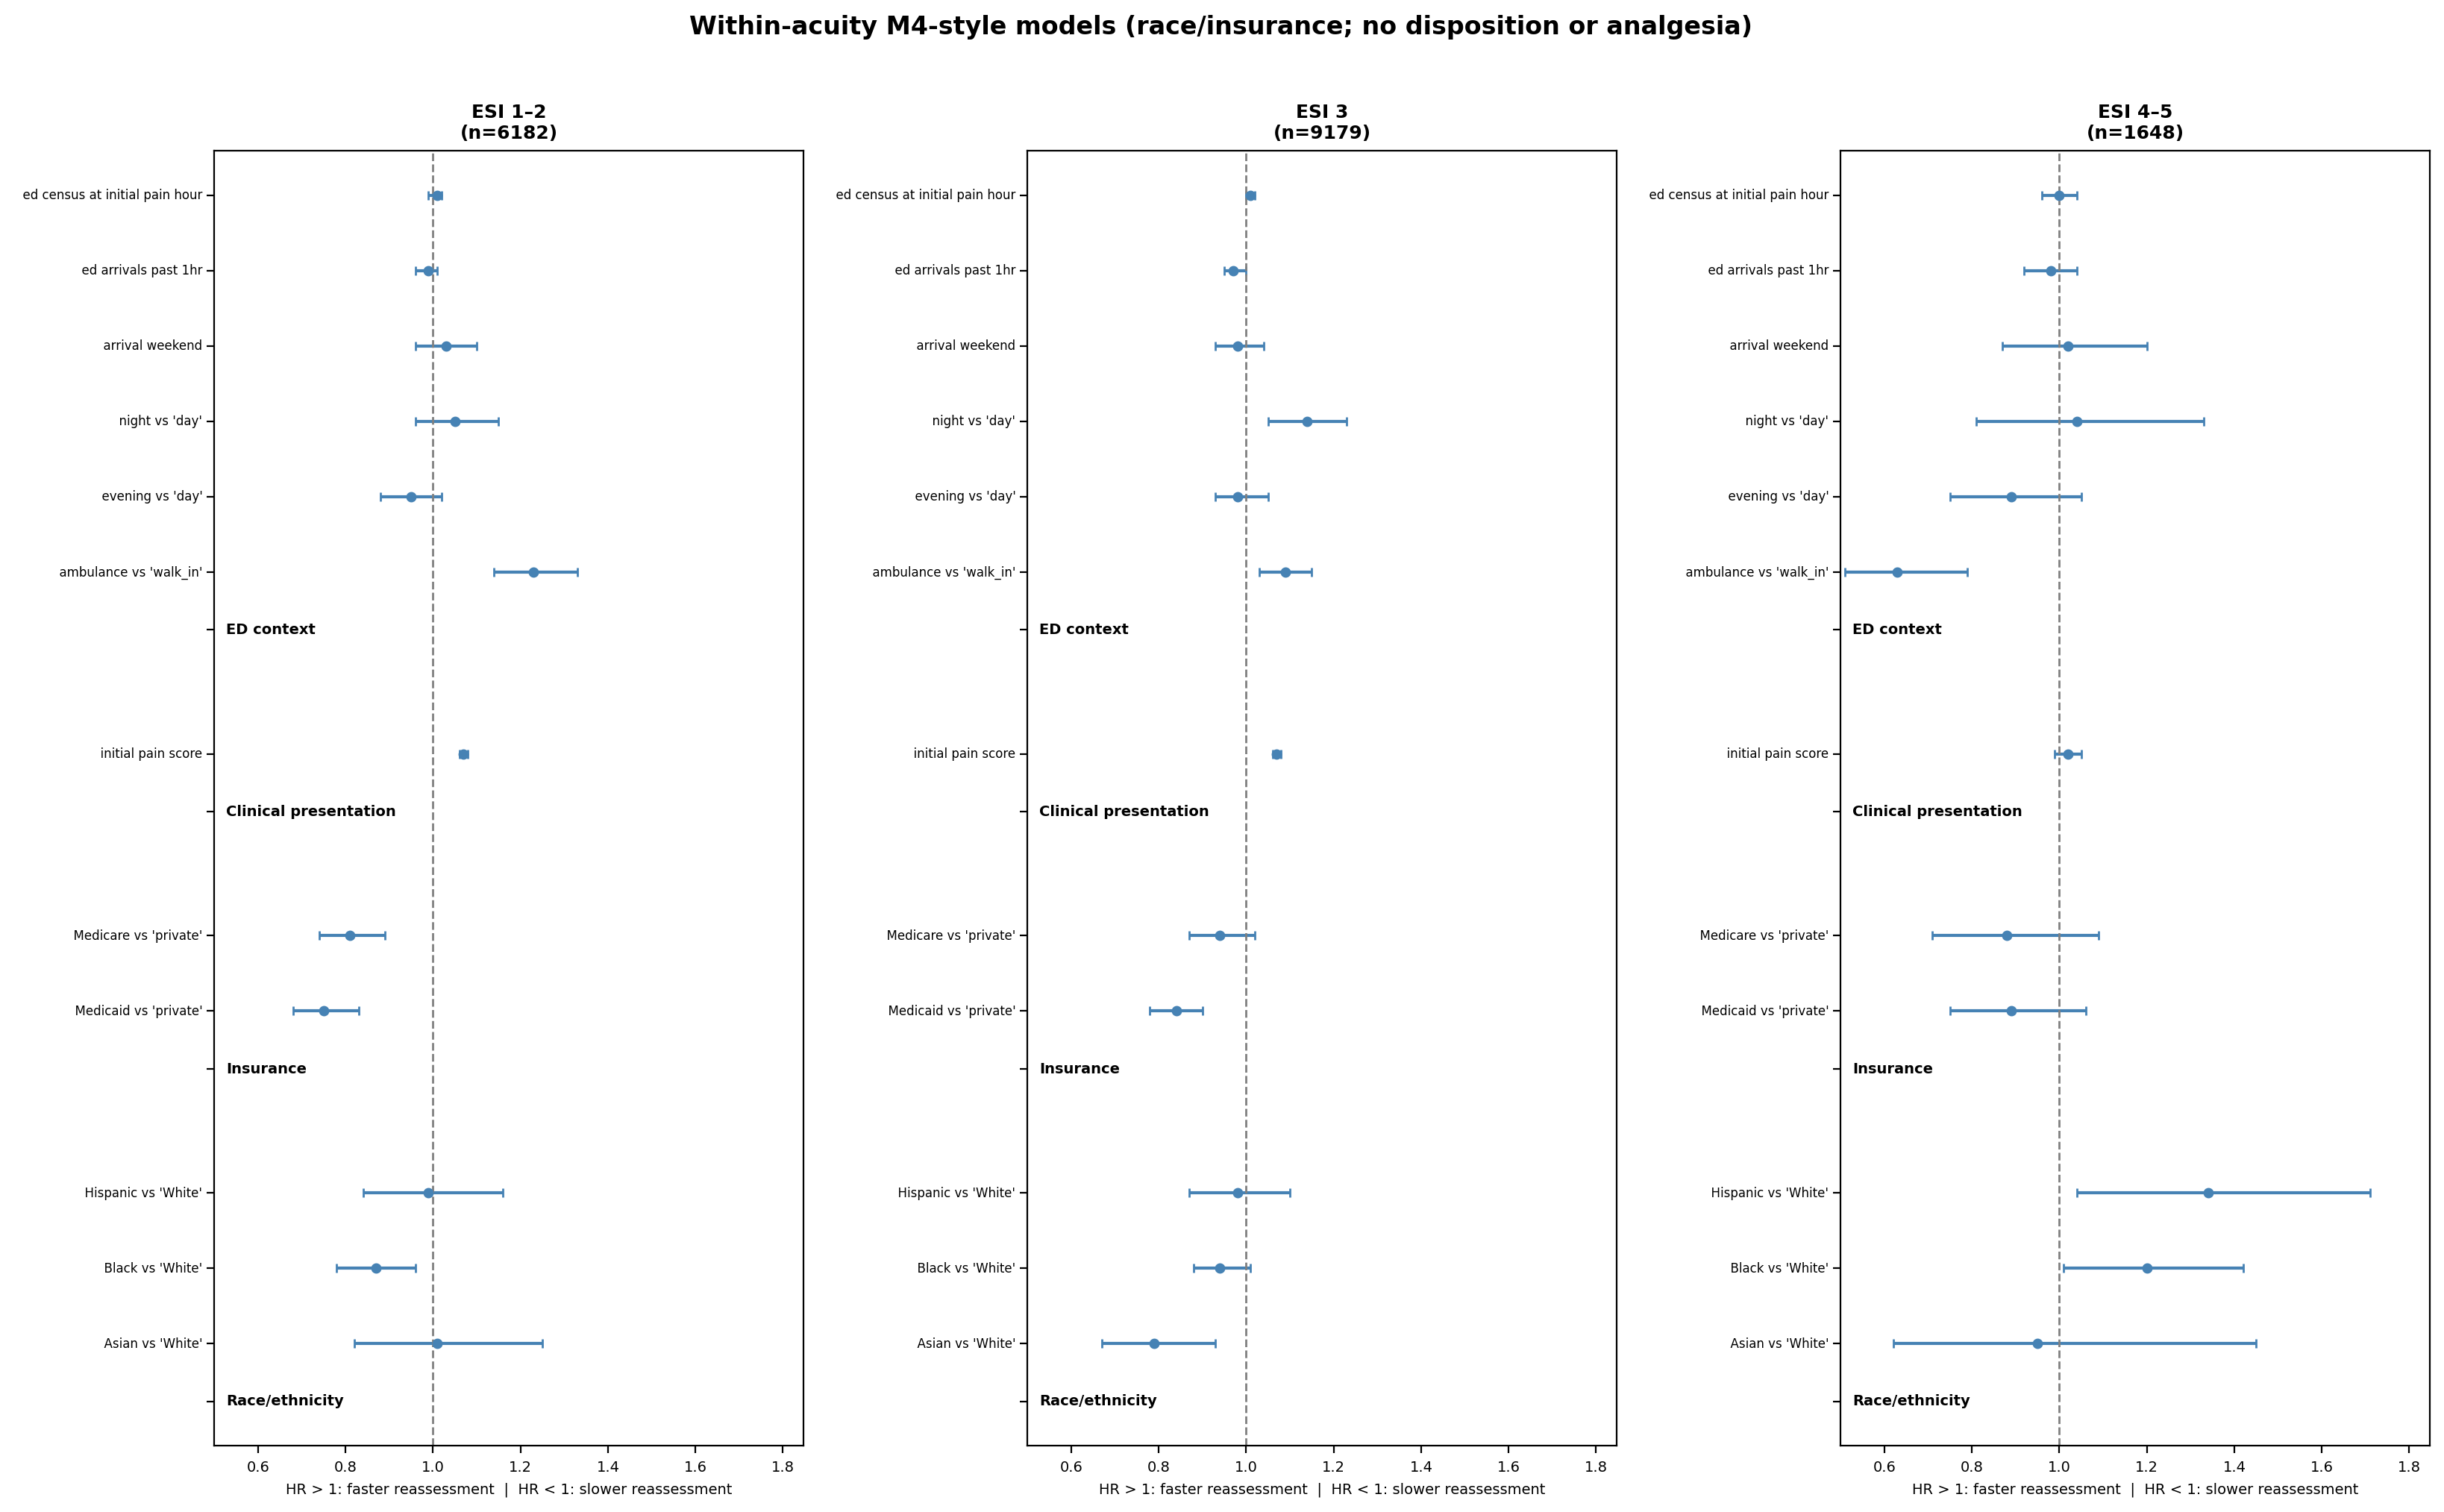
\includegraphics[width=\linewidth]{fig_supp_within_acuity.png}
  \caption{Within-acuity M4-style models: race/ethnicity and insurance by ESI stratum.}
  \label{fig:withinacuity}
\end{figure}

\begin{figure}[htbp]
  \centering
  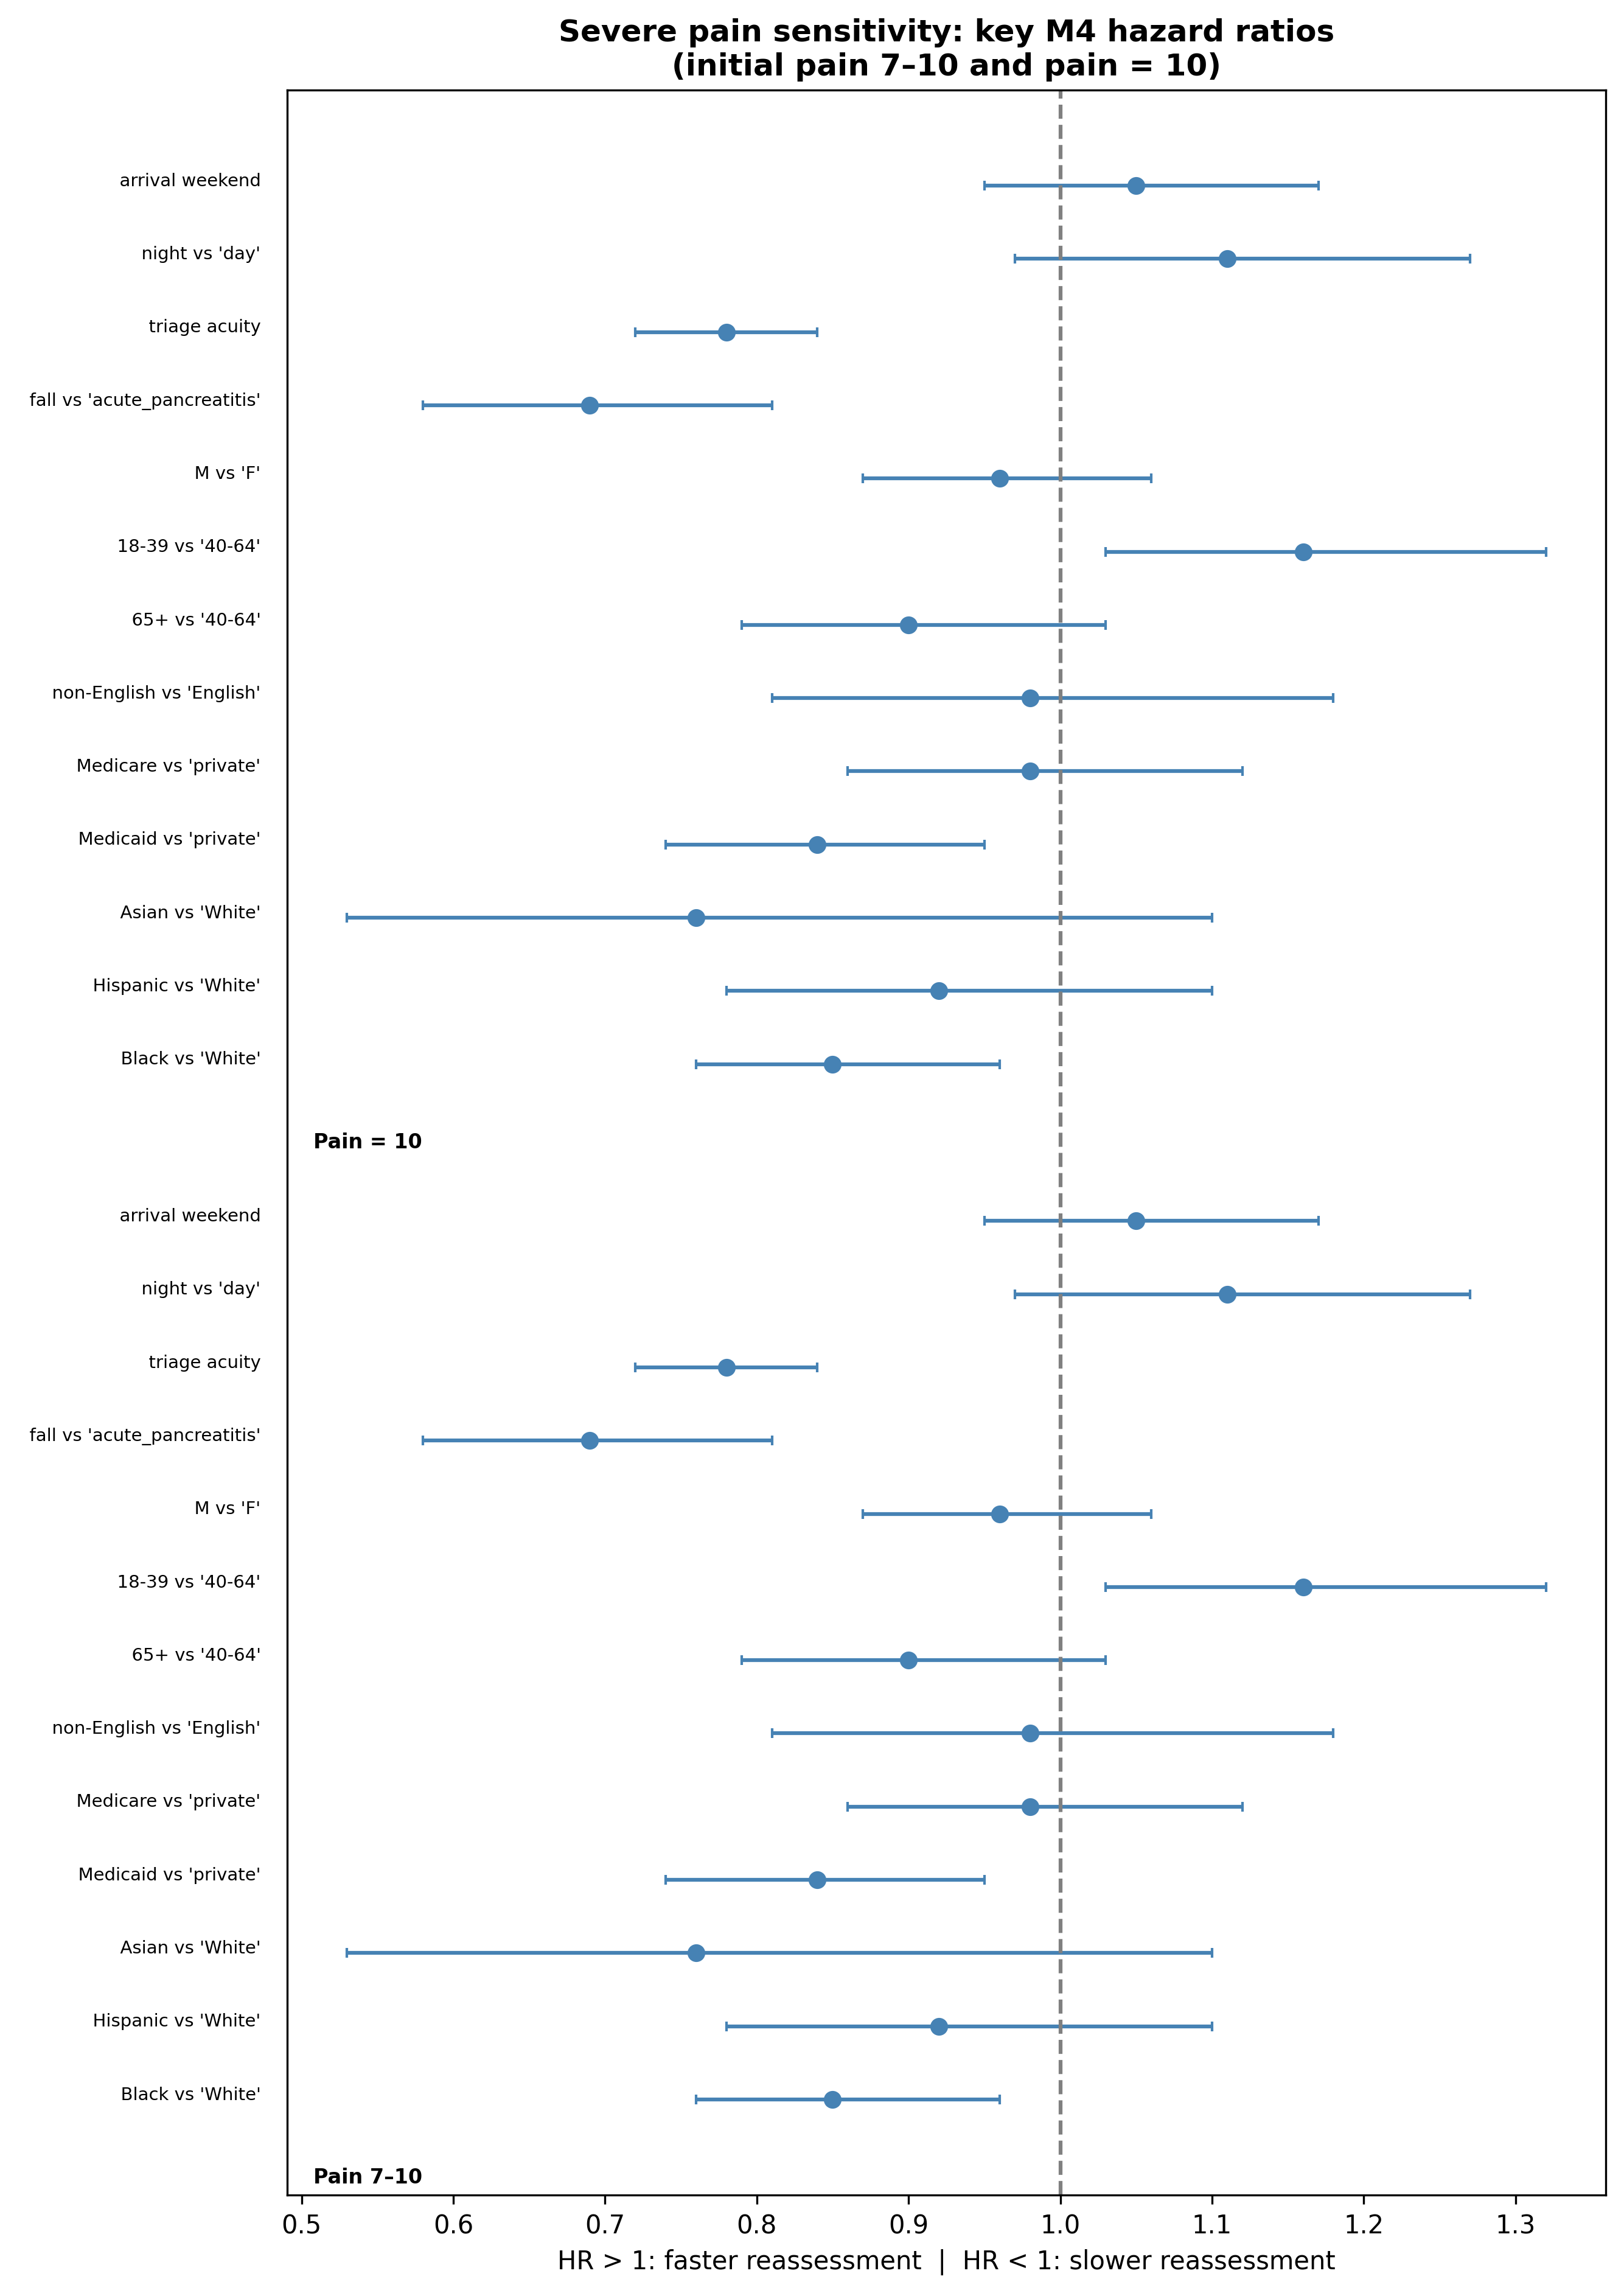
\includegraphics[width=0.95\linewidth]{fig_supp_severe_pain.png}
  \caption{Severe-pain sensitivity analysis (pain 7--10): key M4 hazard ratios.}
  \label{fig:severe}
\end{figure}

\subsection{Competing-risk sensitivity analysis}

In the Fine--Gray model treating ED departure without reassessment as a competing event, results were concordant with the primary Cox model.
Medicaid (sHR \SHRMedicaidFG{}) and Medicare (sHR \SHRMedicareFG{}) remained associated with slower reassessment relative to private insurance, and the Black--White association (sHR \SHRBlackFG{}) was consistent with the primary analysis.
Higher initial pain score (sHR \SHRPainFG{}) and ambulance arrival (sHR \SHRAmbulanceFG{}) remained associated with faster reassessment.
Differential ED departure before reassessment therefore does not explain the observed insurance or race/ethnicity associations (Supplementary Table~\ref{tab:finegray}; Supplementary Figure~\ref{fig:finegray_cif}).

\subsection{Temporal trends}

There was no evidence of a meaningful change in reassessment rates over the study period.
In a supplementary Cox model with continuous de-identified year, the HR per 5-year increase was \HRYearFive{}.
Figure~\ref{fig:yeartrend} displays unadjusted and M4-adjusted probabilities of 60-minute reassessment by policy era; both series fluctuated between approximately 7\% and 12\% without a consistent directional pattern.
Reassessment practices did not improve over the observation window despite national emphasis on pain management quality during this interval.

\begin{figure}[htbp]
  \centering
  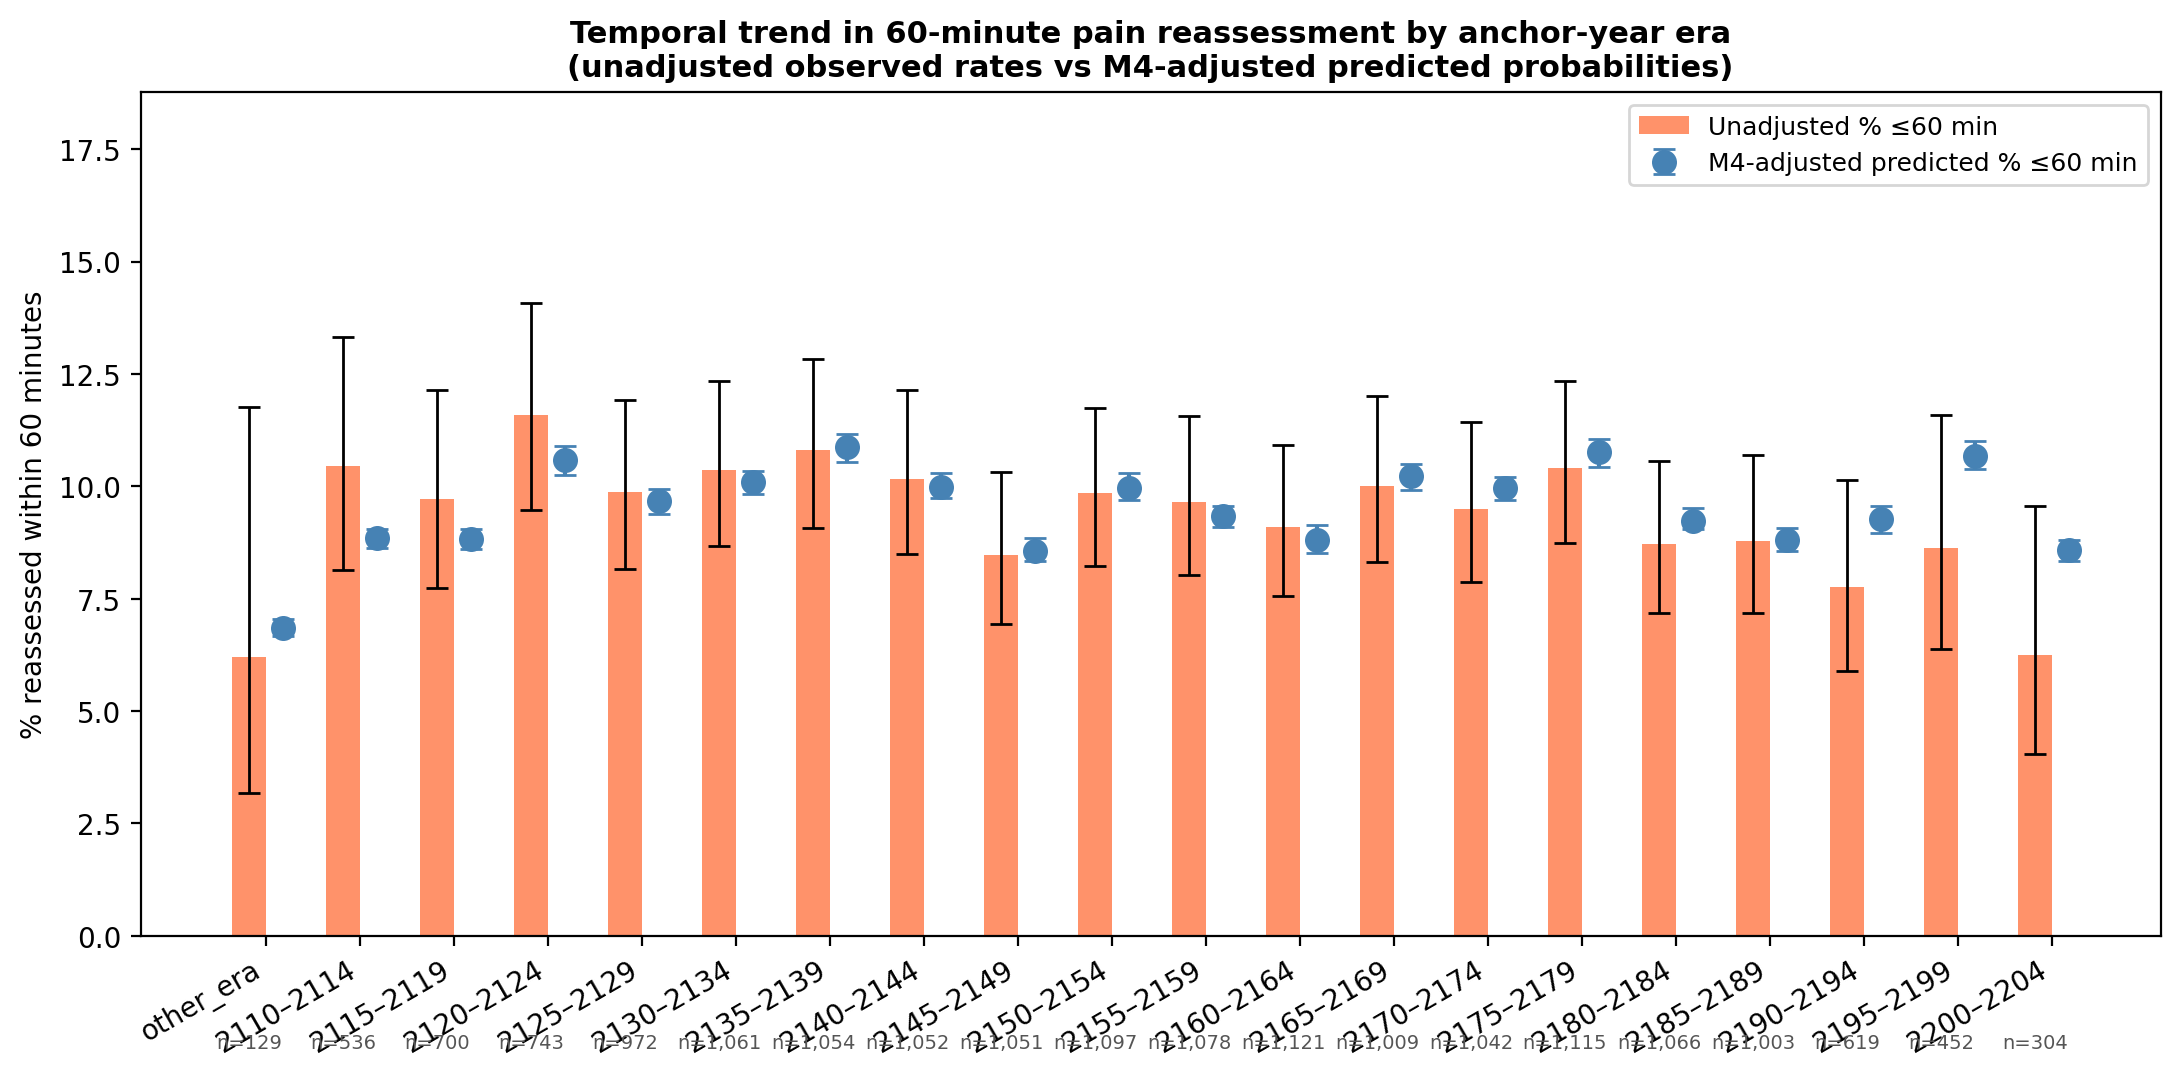
\includegraphics[width=0.95\linewidth]{fig_supp_temporal_trends.png}
  \caption{Year-over-year trends in 60-minute reassessment by de-identified policy era: unadjusted observed rates (bars) and M4-adjusted predicted probabilities (points) with 95\% confidence intervals.}
  \label{fig:yeartrend}
\end{figure}

\subsection{Post-analgesic pathway analysis}

When time zero was reset to the first analgesic administration, cumulative reassessment curves by race/ethnicity largely overlapped and the multivariate log-rank test was not statistically significant in the primary trauma severe-pain subgroup (Figure~\ref{fig:postrx}).
This finding suggests that the demographic patterns observed in the primary analysis, particularly the race and ethnicity associations, are not primarily driven by differences in how quickly patients are monitored after receiving treatment.
The smaller size of this subgroup limits statistical power, and a null log-rank test does not establish equivalence.
The earlier-encounter phase (between initial pain documentation and first reassessment, irrespective of treatment) appears to be where differences in clinical attention emerge.

\begin{figure}[htbp]
  \centering
  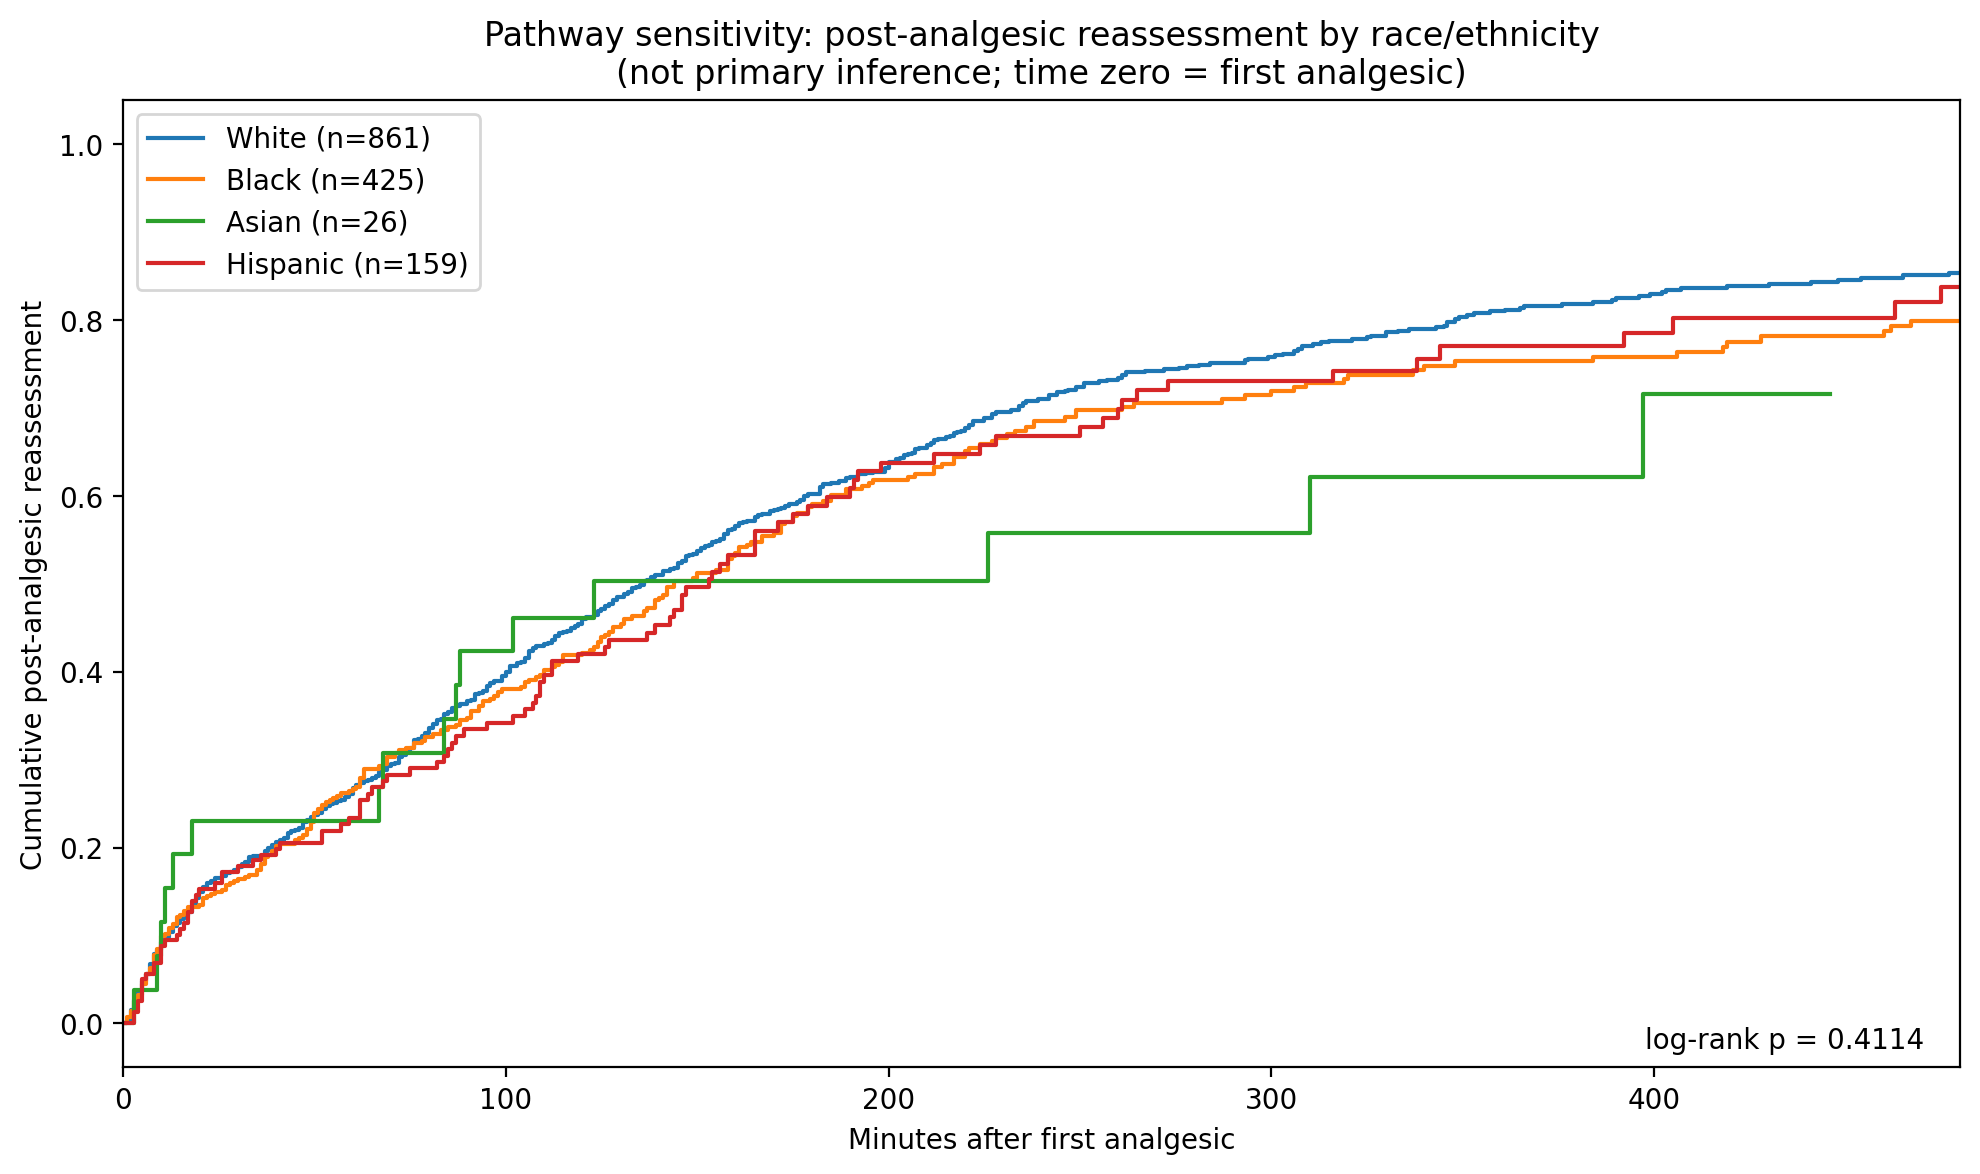
\includegraphics[width=0.85\linewidth]{fig_supp_postanalgesic.png}
  \caption{Post-analgesic pathway sensitivity: reassessment by race/ethnicity with time zero at first analgesic administration.}
  \label{fig:postrx}
\end{figure}


\section{Discussion}
\label{sec:discussion}

In this retrospective cohort of ED encounters with documented pain assessments, we asked how the emergency department responds to a patient's reported pain.
Reassessment was frequently delayed: fewer than one in ten patients had their pain reassessed within 60 minutes of initial documentation, and the median time to reassessment exceeded three hours.
Two findings organize the results.
First, the most robust difference was slower documented reassessment among Medicaid-insured patients compared with privately insured patients, which persisted after adjustment for pain severity, triage acuity, and workflow factors, within acuity strata, among patients reporting severe pain, and in competing-risk analysis.
Second, race and ethnicity differences were present earlier in the care pathway but appeared to be partly embedded in triage and workflow processes rather than persisting as independent associations.

\subsection{The clinical response to pain is shaped by severity, but incompletely}

The strongest and most clinically expected associations were with the pain report itself and with triage acuity.
Patients who reported higher pain were reassessed more quickly; patients assigned lower ESI acuity were reassessed more slowly.
This pattern is broadly consistent with appropriate clinical prioritization: the emergency department allocates monitoring attention in proportion to perceived urgency.
Night-shift associations likely reflect lower census conditions that facilitate more frequent patient contact.

However, the aggregate reassessment rates in this cohort suggest that even among patients with high reported pain, timely reassessment is not the norm.
Only 9.6\% of patients were reassessed within 60 minutes.
If the system is responding appropriately to a pain signal, this baseline rate warrants attention as a quality benchmark independent of any disparity analysis.

\subsection{ESI attenuation as a marker of a disparity mechanism}

An important interpretive point in this paper concerns what the attenuation of race and ethnicity coefficients across sequential models actually means.
Black patients had slower reassessment than White patients in models adjusted only for clinical presentation and demographics.
This association attenuated substantially after adding ESI triage acuity and severity covariates.
A naive reading of this pattern would conclude that the disparity disappears once clinical factors are controlled, and that no inequity remains once case mix is accounted for.
Under the structure hypothesized in Figure~\ref{fig:dag}, that reading is premature, and the distinction matters for how findings like these get translated into policy.

ESI triage acuity is not a neutral measure of objective clinical severity.
It is a judgment, made by a provider, about how urgently a patient's presentation requires attention.
That judgment is susceptible to the same implicit biases documented in pain treatment, analgesic prescribing, and clinical assessment more broadly \citep{Pletcher2008,Anderson2009}.
Empirical evidence supports this: studies have found that Black patients are more likely to be triaged to lower-acuity or fast-track areas relative to White patients with equivalent presenting complaints \citep{Vigil2014,Pines2009}, and that the ESI instrument relies on subjective determinations, particularly resource prediction, that are prone to unintentional racial bias \citep{Fernandes2005}.
When a Black patient and a White patient present with the same pain score and the same diagnosis, and receive different ESI assignments, those assignments carry the difference forward into every downstream outcome that ESI predicts, including reassessment timing.

To the extent that ESI acts as a pathway variable rather than a confounder, adjustment does more than remove confounding; it also removes part of the association of interest.
The attenuation of the Black--White coefficient from M2 to M3 is therefore consistent with differential triage assignment as a possible mechanism through which racial differences in reassessment arise.
It should not be read as evidence that the disparity is explained away.
Because M3 adds severity covariates alongside ESI, and because these sequential models do not constitute a formal mediation analysis, the attenuation cannot be apportioned to ESI specifically.
The residual M4 coefficient represents the association not accounted for by measured triage and workflow variables, not the total difference between groups; estimates that do not adjust for ESI would show larger and more persistent race/ethnicity associations.

This distinction matters for intervention design.
If racial differences in reassessment operate partly through triage assignment, then interventions that target downstream monitoring protocols without addressing triage equity may be insufficient.
The triage process itself, the point at which a provider encodes their assessment of urgency, is a plausible site where such differences arise.

\subsection{Insurance: an association not explained by the measured care pathway}

The clearest signal of uneven pain monitoring in this study comes from the persistence of the Medicaid--private difference among patients reporting severe pain.
Among patients with initial pain scores of 7--10, Medicaid patients were still reassessed substantially more slowly than privately insured patients (HR \HRMedicaidSevere{}).
These patients have already cleared the threshold that should, on clinical grounds alone, prompt monitoring: they reported severe pain at triage.
The insurance gradient that persists in this subgroup is therefore not attributable to Medicaid patients appearing lower-acuity, reporting lower pain, or being clinically less urgent.
It reflects something in the care encounter itself that is associated with payer status and that shapes how often patients are checked on.

Across the full cohort, the Medicaid association showed minimal attenuation from M2 through M4, in contrast to the race and ethnicity findings, and was unchanged when ED departure without reassessment was treated as a competing event.
Medicaid patients were reassessed approximately 20\% more slowly than privately insured patients at the same triage level, with the same initial pain score, arriving by the same mode, during the same shift.
Within-acuity analyses confirm this pattern persists even among ESI 1--2 patients (HR \HRMedicaidESIhigh{}), those whose triage designation explicitly signals the highest clinical urgency.
The persistence of this association suggests that Medicaid status captures social, structural, or care-process factors not measured in this dataset.
These findings identify Medicaid status as a robust marker of slower documented reassessment, but they do not establish whether payer status itself directly influenced bedside clinician behavior.

The candidate mechanisms are plausible but unmeasured: differences in how nursing attention is distributed across patients, in how assertively patients advocate for themselves, in implicit provider assumptions about which patients require close monitoring, or in structural factors such as bed assignment and staffing ratios that correlate with payer mix at the unit level.
Distinguishing among these mechanisms requires prospective data beyond what administrative records can provide.

What administrative data can establish, and what this study does establish, is that the association is consistent across model specifications and is not attributable to measured clinical or operational factors.
Because reassessment is directly observable, protocol-adjacent, and less dependent on subjective clinical judgment than treatment selection, it is a more tractable quality-improvement target than treatment disparities.
Structured reassessment protocols tied to ESI level, nursing workflow checklists, and electronic alerts for time since last pain documentation are all interventions that operate at the level where this difference appears to arise.

\subsection{Temporal stability}

Reassessment rates did not improve meaningfully across the study period, despite national emphasis on pain management quality during this interval.
Both unadjusted and adjusted estimates of 60-minute reassessment fluctuated between approximately 7\% and 12\% without directional improvement across policy eras.
This stability suggests that reassessment documentation practices were not materially affected by broader quality initiatives.
These results motivate explicit inclusion of reassessment metrics in future quality measurement frameworks.

\subsection{Limitations}

This study has several important limitations.
Data come from a single academic medical center via MIMIC-IV-ED; findings may not generalize to community or safety-net EDs, which may have different staffing structures, patient populations, and documentation practices.
The cohort was restricted to acute pancreatitis and trauma diagnoses; findings should not be extrapolated to all ED pain presentations.
Pain scores and reassessment timestamps reflect documentation behavior, which may differ from the underlying clinical activity: a nurse who checks on a patient but does not document a pain score would not contribute a reassessment event in this analysis.
We could not fully account for analgesic timing, provider-level variation, or patient advocacy behaviors that may mediate or moderate the associations we observe.
Comorbidity measurement depended on linked ICD flags, which may be incomplete.
We also could not determine whether insurance status was visible to bedside clinicians at the time of care; insurance-based differences should therefore be interpreted as associations with a social and structural marker rather than evidence that payer status directly altered clinician behavior.
Unmeasured patient-level factors that differ by payer, such as chronic opioid therapy, behavioral health comorbidity, housing instability, or prior utilization patterns, may confound the insurance association and cannot be excluded with these data.
De-identified calendar years prevent direct mapping to specific policy interventions or institutional changes.
Finally, interpretation of the sequential model coefficients depends on the hypothesized framework in Figure~\ref{fig:dag}; if ESI assignment is influenced by unmeasured variables that also affect reassessment, the structural interpretation of the attenuation pattern may be incorrect.
The competing-risk sensitivity analysis addresses informative censoring at ED departure and produced concordant results, but other forms of informative censoring cannot be fully excluded.

\subsection{Conclusions}

Three findings summarize this study.
First, pain reassessment was infrequent and delayed overall: fewer than one in ten patients were reassessed within 60 minutes, identifying a quality gap that precedes any consideration of disparities.
Second, the most robust difference was by insurance status: Medicaid status remained a strong marker of slower documented reassessment across clinical, triage, workflow, severe-pain, within-acuity, and competing-risk analyses, and the mechanism is not measured in these data.
Third, race and ethnicity differences were less consistent as independent associations and may instead be partly embedded in triage and workflow pathways, implicating acuity assignment as a candidate site where such differences arise.
Pain reassessment should be considered alongside analgesic outcomes in quality assessment.
Future work should validate these associations in multi-center cohorts, link reassessment timing to patient-reported pain outcomes, and evaluate targeted interventions to standardize reassessment across payer groups and triage strata.



\begin{thebibliography}{10}
\bibitem[Anderson et~al.(2009)]{Anderson2009} Anderson KO, Green CR, Payne R. Racial and ethnic disparities in pain: causes and consequences of unequal care. \emph{J Pain}. 2009;10(12):1187--1204.
\bibitem[Fernandes et~al.(2005)]{Fernandes2005} Fernandes CMB, Tanabe P, Gilboy N, et~al. Five-level triage: a report from the ACEP/ENA five-level triage task force. \emph{J Emerg Nurs}. 2005;31(1):39--50.
\bibitem[Fine and Gray(1999)]{Fine1999} Fine JP, Gray RJ. A proportional hazards model for the subdistribution of a competing risk. \emph{J Am Stat Assoc}. 1999;94(446):496--509.
\bibitem[Johnson et~al.(2023)]{Johnson2023MIMICIVED} Johnson AEW, Bulgarelli L, Shen L, et~al. MIMIC-IV-ED: an emergency department dataset. \emph{Sci Data}. 2023;10:409.
\bibitem[Meltzer et~al.(2014)]{Meltzer2014} Meltzer AC, Pines JM, Richards LM, Mullins PM, Mazer-Amirshahi M. US emergency department visits for adults with mental health disorders. \emph{Psychiatr Serv}. 2014;65(6):811--814.
\bibitem[Pines et~al.(2009)]{Pines2009} Pines JM, Iyer S, Disbot M, Hollander JE, Shofer FS, Datner EM. The effect of emergency department crowding on patient satisfaction for admitted patients. \emph{Acad Emerg Med}. 2009;15(9):825--831.
\bibitem[Pletcher et~al.(2008)]{Pletcher2008} Pletcher MJ, Kertesz SG, Kohn MA, Gonzales R. Trends in opioid prescribing by race/ethnicity for patients seeking care in US emergency departments. \emph{JAMA}. 2008;299(1):70--78.
\bibitem[Todd et~al.(2007)]{Todd2007PEMI} Todd KH, Ducharme J, Choiniere M, et~al. Pain in the emergency department: results of the pain and emergency medicine initiative (PEMI) multicenter study. \emph{J Pain}. 2007;8(6):460--466.
\bibitem[Vigil et~al.(2014)]{Vigil2014} Vigil JM, Coulombe P, Alcock J, Kruger E, Stith SS, Sutherland WS. Patient ethnicity influences emergency department analgesia and wait times. \emph{Pain Res Treat}. 2014;2014:1--6.
\bibitem[von Elm et~al.(2007)]{vonElm2007STROBE} von Elm E, Altman DG, Egger M, Pocock SJ, G\"otzsche PC, Vandenbroucke JP. The STROBE statement: guidelines for reporting observational studies. \emph{Lancet}. 2007;370(9596):1453--1457.
\end{thebibliography}


\clearpage
\appendix

% Supplementary materials — included via \appendix in main.tex
\section*{Supplementary Materials}
\addcontentsline{toc}{section}{Supplementary Materials}
\label{sec:supplement}
\setcounter{figure}{0}
\renewcommand{\thefigure}{S\arabic{figure}}
\setcounter{table}{0}
\renewcommand{\thetable}{S\arabic{table}}

Code to reproduce all analyses and figures is available in the study repository (\texttt{scripts/run\_analysis.py}).

\begin{table}[htbp]
  \centering
  \caption{\textbf{Supplementary Table S1.} Vital-sign hazard ratios from the M4 model.
  Initial heart rate, respiratory rate, and systolic blood pressure (each z-scored) are adjusted for in M3 and M4 but are not displayed in the primary forest plot (Figure~\ref{fig:m4forest} in main text).
  HR per one standard-deviation increase in each vital sign.}
  \label{tab:vitals_supp}
  \footnotesize
  \begin{tabular}{@{}lcc@{}}
    \toprule
    Vital sign (z-scored) & HR (95\% CI) & $p$-value \\
    \midrule
    Heart rate & 1.03 (1.00--1.05) & 0.019 \\
    Respiratory rate & 1.01 (1.00--1.02) & 0.082 \\
    Systolic blood pressure & 0.99 (0.98--1.01) & 0.575 \\
    \bottomrule
  \end{tabular}
\end{table}

\begin{figure}[htbp]
  \centering
  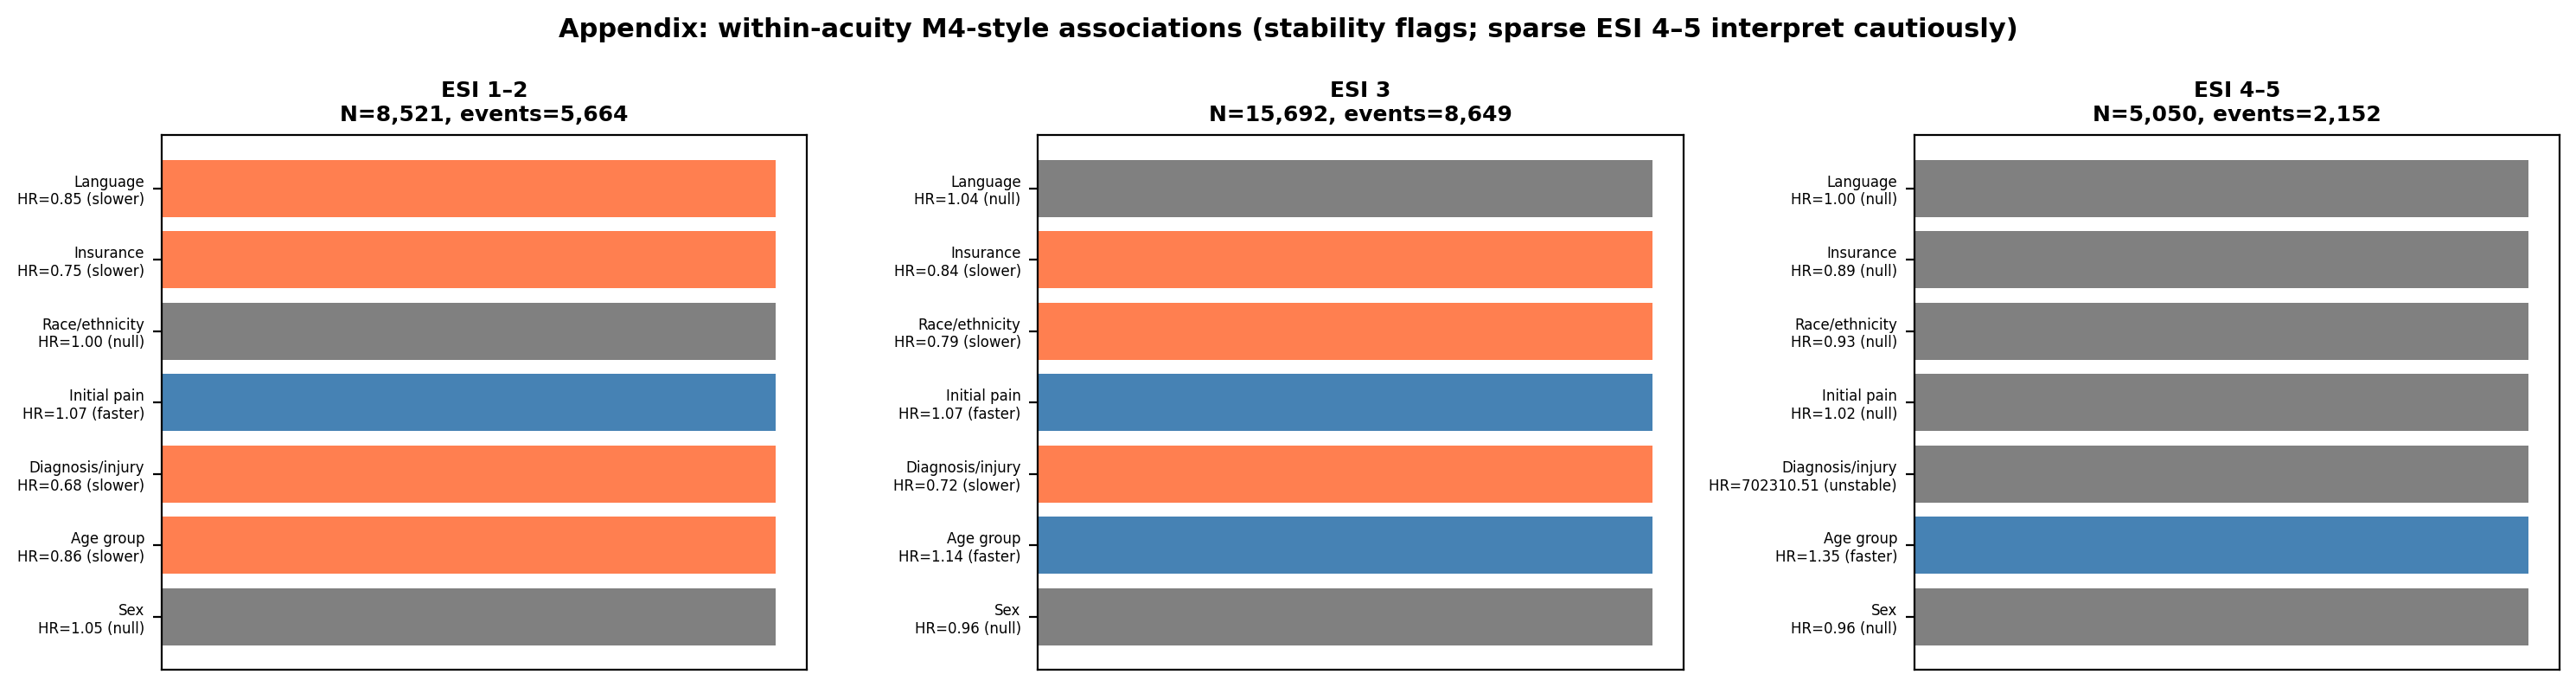
\includegraphics[width=\linewidth]{fig_within_acuity_age_sex_diagnosis_pain.png}
  \caption{\textbf{Supplementary Figure S2.} Within-acuity M4-style associations for age, sex, diagnosis, and language (stability flags; sparse ESI 4--5 strata should be interpreted cautiously).
  Complements main-text within-acuity results for insurance and race/ethnicity (Figure~\ref{fig:withinacuity}).}
  \label{fig:acuity_heatmap}
\end{figure}

\begin{figure}[htbp]
  \centering
  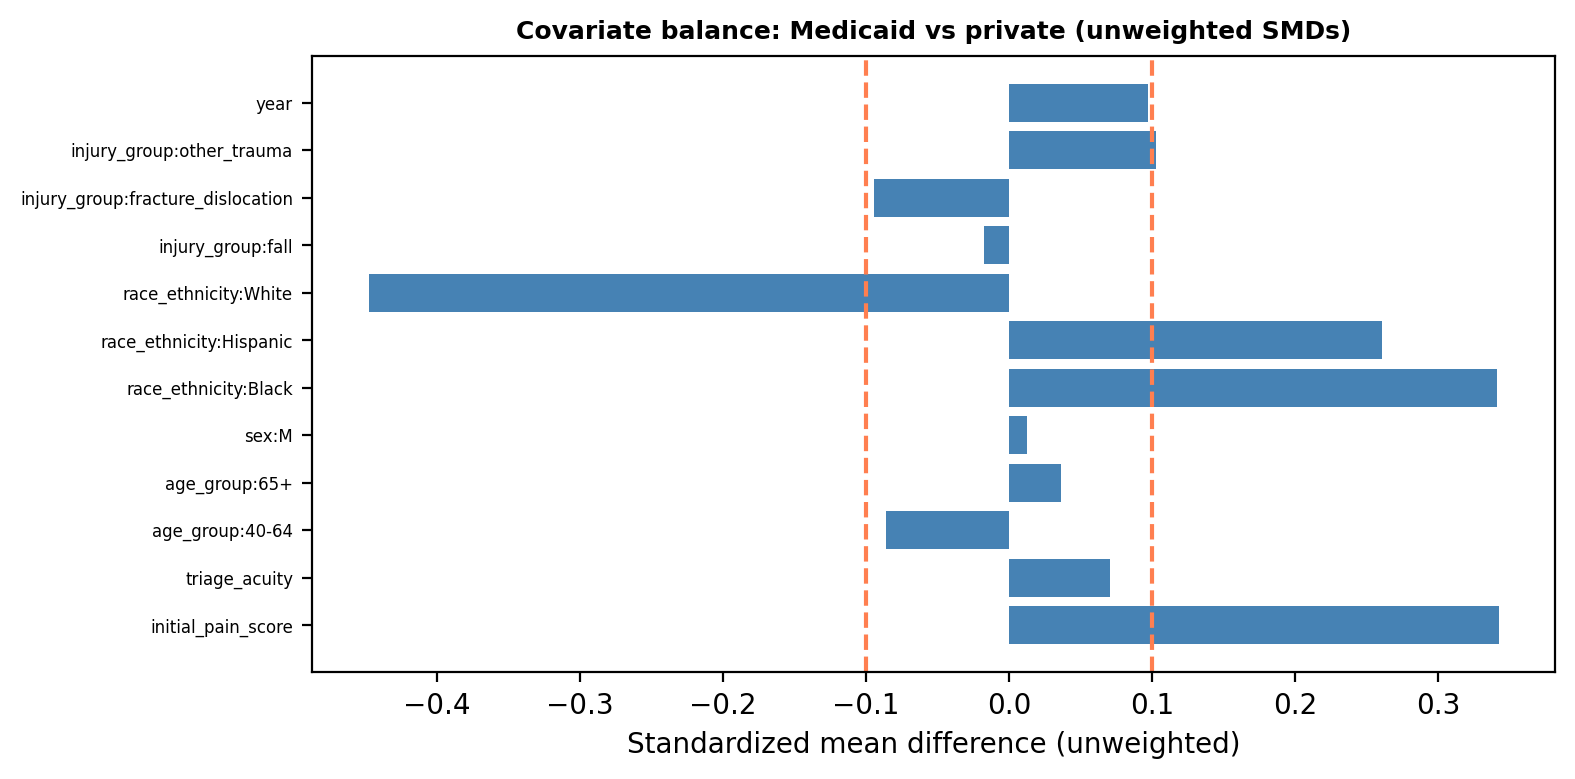
\includegraphics[width=0.85\linewidth]{fig_iptw_balance_medicaid_private.png}
  \caption{\textbf{Supplementary Figure S3.} Covariate balance for Medicaid vs.\ private (unweighted standardized mean differences).
  Standardized mean differences before inverse probability of treatment weighting (IPTW), using propensity scores estimated from M1--M3 covariates.}
  \label{fig:iptw_balance}
\end{figure}

\begin{figure}[htbp]
  \centering
  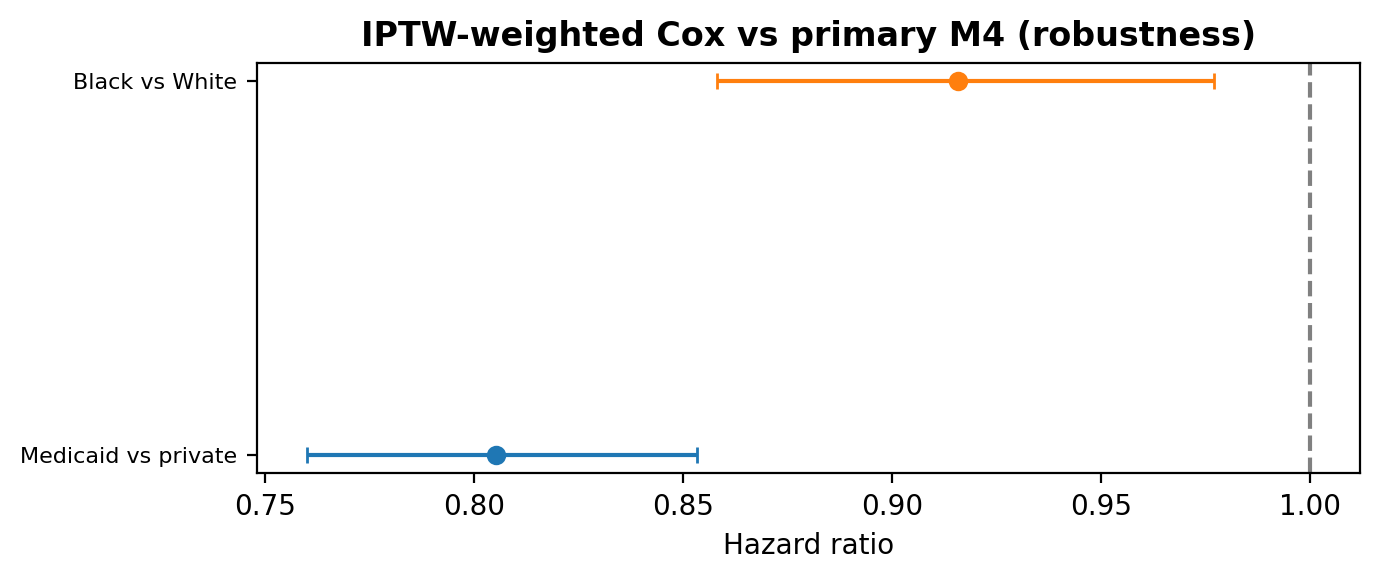
\includegraphics[width=0.85\linewidth]{fig_iptw_weighted_cox_results.png}
  \caption{\textbf{Supplementary Figure S4.} IPTW-weighted Cox vs.\ primary M4 (robustness).
  Weighted hazard ratio for Medicaid vs.\ private insurance compared with the unweighted M4 estimate.}
  \label{fig:iptw_cox}
\end{figure}

\begin{figure}[htbp]
  \centering
  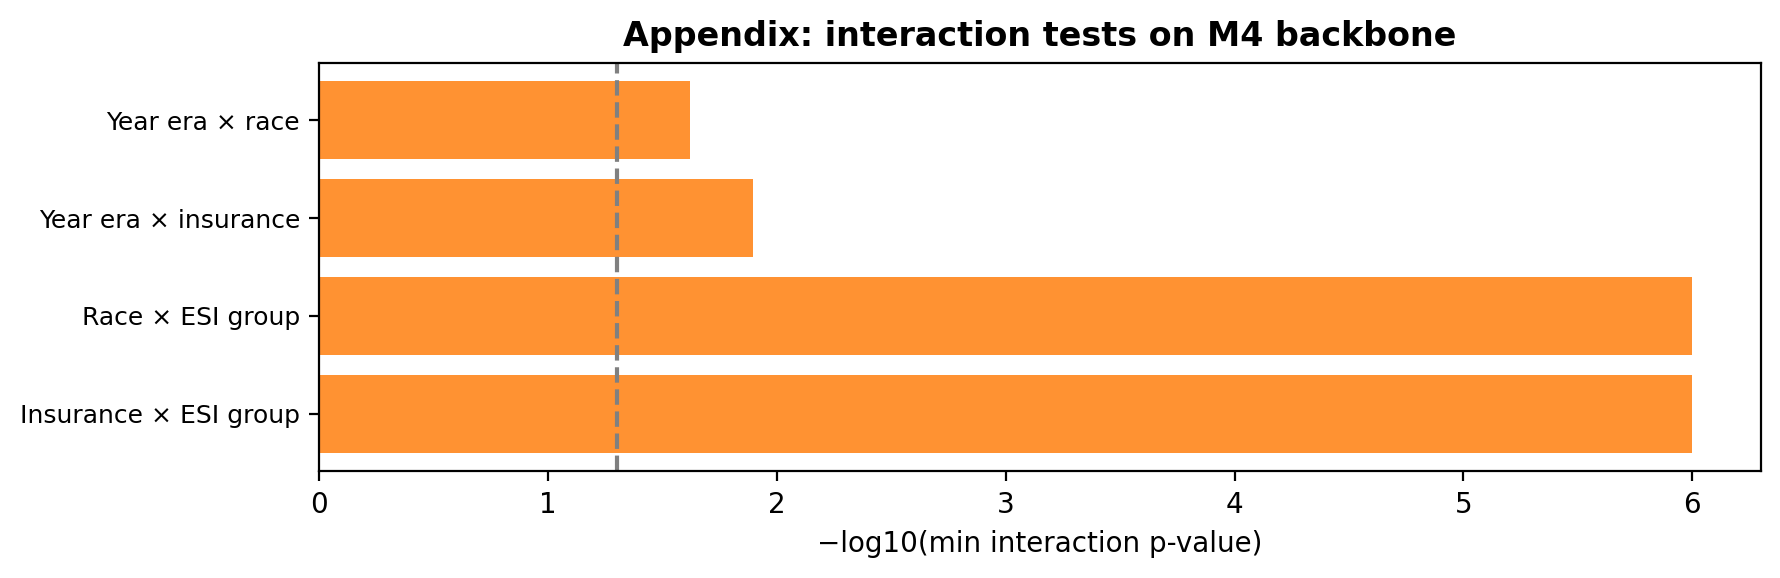
\includegraphics[width=0.85\linewidth]{figA_interaction_summary.png}
  \caption{\textbf{Supplementary Figure S5.} Interaction tests on the M4 backbone.
  Race~$\times$~ESI, insurance~$\times$~ESI, and year-era interaction terms on the M4 covariate set.}
  \label{fig:interactions_supp}
\end{figure}

\subsection*{Supplementary: Competing-risk sensitivity analysis (Fine--Gray)}

The primary Cox model censors patients without reassessment at ED departure, which assumes that departure is non-informative with respect to the reassessment process.
To test whether differential early departure rates bias the primary estimates, we fit a Fine--Gray subdistribution hazard model \citep{Fine1999} treating ED departure without reassessment as a competing event.
The full M4 covariate set was used; analysis was conducted in R~4.5.2 (\texttt{cmprsk} package v2.2.12).
The model was fit on \num{17009} complete cases; the \num{195} encounters excluded relative to the primary cohort (\CohortN{}) had missing values in one or more M4 covariates required by the competing-risk design matrix.

\begin{table}[htbp]
  \centering
  \caption{\textbf{Supplementary Table S2.} Fine--Gray subdistribution hazard model: full M4 covariate set.
  Event of interest: first pain reassessment; competing event: ED departure without reassessment.
  sHR $>1$: faster subdistribution hazard (more rapid reassessment); sHR $<1$: slower.
  $n=\num{17009}$ complete cases.}
  \label{tab:finegray}
  \begin{tabular}{lrrr}
\toprule
Covariate & sHR & 95\% CI & $p$ \\
\midrule
\multicolumn{4}{l}{\textit{Clinical presentation}} \\
Initial pain score & 1.10 & 1.10--1.11 & $<$0.001 \\
Injury: fall vs.\ AP & 0.79 & 0.73--0.85 & $<$0.001 \\
Injury: fracture/dislocation vs.\ AP & 0.85 & 0.77--0.94 & 0.002 \\
Injury: other trauma vs.\ AP & 0.74 & 0.69--0.80 & $<$0.001 \\
\midrule
\multicolumn{4}{l}{\textit{Demographics \& social factors}} \\
Race: Asian vs.\ White & 0.92 & 0.81--1.04 & 0.17 \\
Race: Black vs.\ White & 0.89 & 0.84--0.94 & $<$0.001 \\
Race: Hispanic vs.\ White & 0.96 & 0.88--1.05 & 0.41 \\
Age: 18--39 vs.\ 40--64 & 0.98 & 0.93--1.04 & 0.48 \\
Age: 65+ vs.\ 40--64 & 1.05 & 1.00--1.11 & 0.063 \\
Sex: male vs.\ female & 0.99 & 0.95--1.03 & 0.50 \\
Insurance: Medicaid vs.\ private & 0.85 & 0.80--0.90 & $<$0.001 \\
Insurance: Medicare vs.\ private & 0.93 & 0.88--0.98 & 0.008 \\
Language: non-English vs.\ English & 0.97 & 0.89--1.05 & 0.43 \\
\midrule
\multicolumn{4}{l}{\textit{Triage \& severity}} \\
ESI triage acuity (per unit) & 0.78 & 0.75--0.80 & $<$0.001 \\
Heart rate (z-scored) & 1.07 & 1.05--1.10 & $<$0.001 \\
Respiratory rate (z-scored) & 1.01 & 1.01--1.01 & $<$0.001 \\
Systolic BP (z-scored) & 1.02 & 1.00--1.04 & 0.082 \\
\midrule
\multicolumn{4}{l}{\textit{ED workflow \& context}} \\
Arrival: ambulance vs.\ walk-in & 1.25 & 1.20--1.31 & $<$0.001 \\
Arrival: other vs.\ walk-in & 0.98 & 0.82--1.18 & 0.83 \\
Shift: evening vs.\ day & 0.99 & 0.95--1.04 & 0.80 \\
Shift: night vs.\ day & 1.11 & 1.05--1.18 & $<$0.001 \\
Weekend arrival & 1.00 & 0.96--1.05 & 0.84 \\
ED arrivals past 1 hr & 1.04 & 1.02--1.06 & $<$0.001 \\
ED census at pain hour & 0.99 & 0.98--1.00 & 0.005 \\
\bottomrule
\end{tabular}

\end{table}

\begin{figure}[htbp]
  \centering
  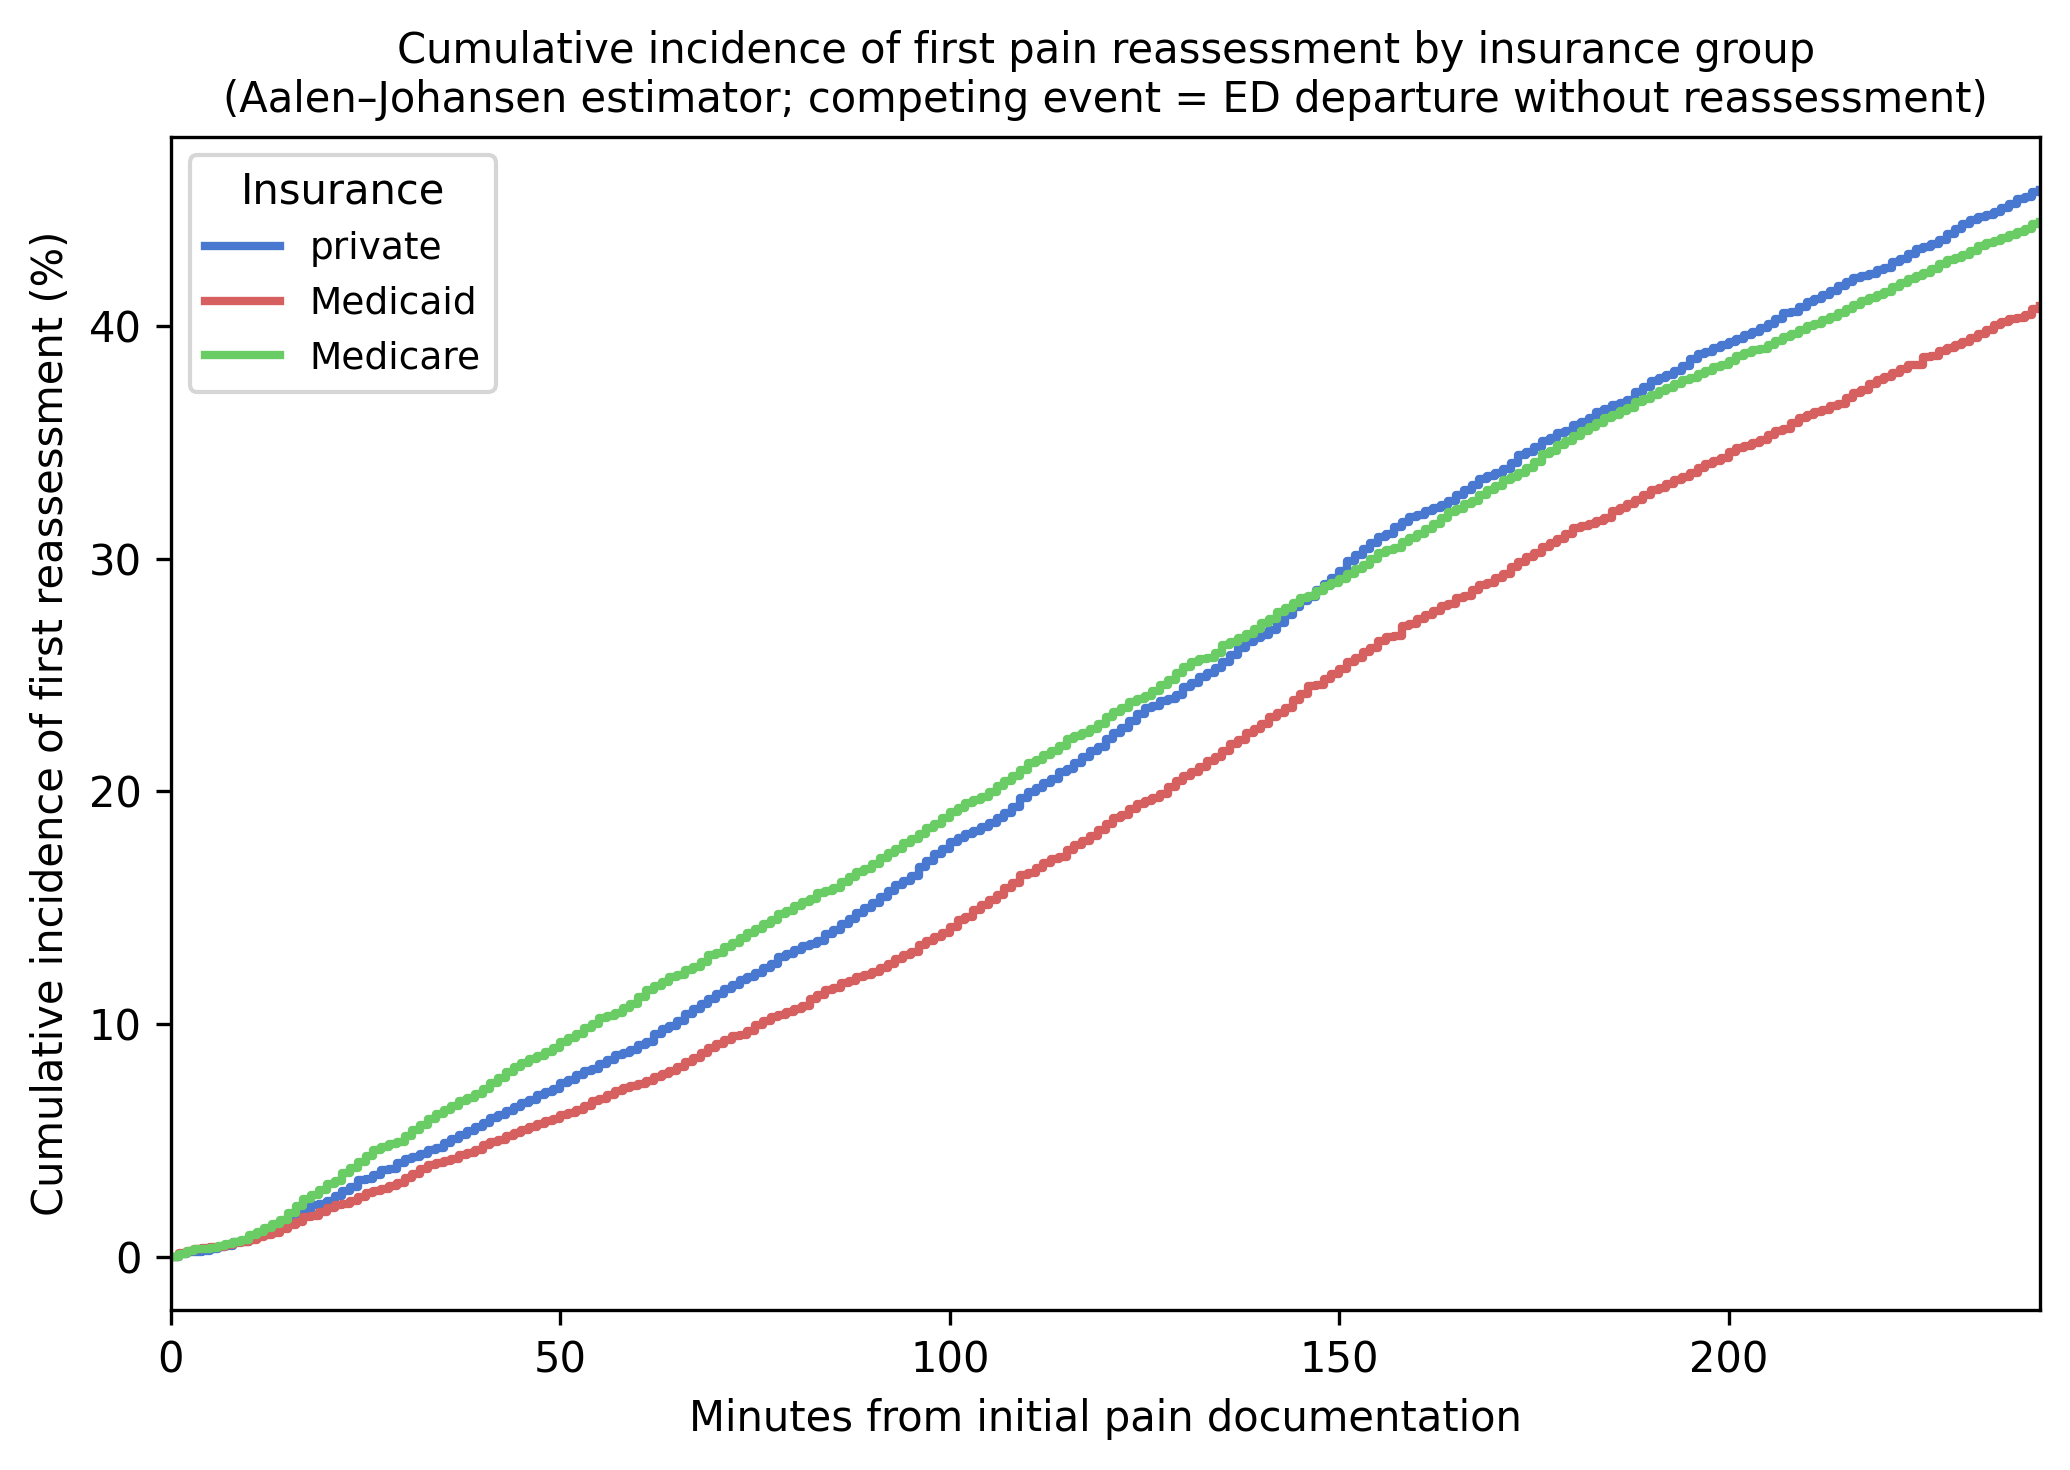
\includegraphics[width=0.85\linewidth]{fig_supp_finegray_cif.png}
  \caption{\textbf{Supplementary Figure S6.} Cumulative incidence of first pain reassessment by insurance group, estimated by the Aalen--Johansen estimator.
  ED departure without reassessment is treated as a competing event.
  Curves show the subdistribution cumulative incidence within 240 minutes of initial pain documentation.}
  \label{fig:finegray_cif}
\end{figure}

The Fine--Gray results were concordant with the primary Cox model.
Medicaid-insured patients showed a significantly lower subdistribution hazard ratio (sHR \SHRMedicaidFG{}) and Medicare-insured patients also showed slower reassessment (sHR \SHRMedicareFG{}), indicating that the insurance association is not explained by differential rates of ED departure before reassessment.
Black patients showed a significantly lower sHR (sHR \SHRBlackFG{}), consistent with the primary analysis.
The only directional discordance was for Hispanic patients (Cox HR 1.04 vs.\ sHR 0.96), but both estimates were non-significant and crossed 1.0, indicating no meaningful difference in either framework.
Overall, these competing-risk results support the robustness of the primary Cox conclusions.


\end{document}
